\documentclass[symmetric, a4paper]{tufte-book}

%% configuration, packages

\usepackage{colortbl} 

\hypersetup{colorlinks}% uncomment this line if you prefer colored hyperlinks (e.g., for onscreen viewing)

%% TODO add logic for quasar / orange name change

\usepackage{import}

%%
% If they're installed, use Bergamo and Chantilly from www.fontsite.com.
% They're clones of Bembo and Gill Sans, respectively.
%\IfFileExists{bergamo.sty}{\usepackage[osf]{bergamo}}{}% Bembo
%\IfFileExists{chantill.sty}{\usepackage{chantill}}{}% Gill Sans

%\usepackage{microtype}

\usepackage{tcolorbox}
\usepackage[english]{babel}

%%
% For nicely typeset tabular material
\usepackage{booktabs}

% For stacking images
\usepackage{stackengine}

\usepackage{wrapfig}
\setlength{\wrapoverhang}{5.5cm} % this is something we can set in future to whatever the exact position is

%%
% For graphics / images
\usepackage{graphicx}
%\setkeys{Gin}{width=\linewidth,totalheight=\textheight,keepaspectratio}  % disabled for problems with scale/resolution
\setkeys{Gin}{keepaspectratio}

\graphicspath{{graphics/}}

% The fancyvrb package lets us customize the formatting of verbatim
% environments.  We use a slightly smaller font.
\usepackage{fancyvrb}
\usepackage{hyperref}
\fvset{fontsize=\normalsize}

%%
% Sets the name of the package between Orange compilations
% Always use this instead of directly referring to Orange or Quasar or Oasys, etc.
\newcommand{\mutation}{Orange}
% \newcommand{\mutation}{scOrange}
% \newcommand{\mutation}{Quasar}
\newcommand{\widget}[1]{\textsl{#1}}
\newcommand{\wn}{~cm$^{-1}$}

%%
% Prints argument within hanging parentheses (i.e., parentheses that take
% up no horizontal space).  Useful in tabular environments.
\newcommand{\hangp}[1]{\makebox[0pt][r]{(}#1\makebox[0pt][l]{)}}

%%
% Prints an asterisk that takes up no horizontal space.
% Useful in tabular environments.
\newcommand{\hangstar}{\makebox[0pt][l]{*}}

%%
% Prints a trailing space in a smart way.
\usepackage{xspace}

\newcommand{\TL}{Tufte-\LaTeX\xspace}

% Prints the month name (e.g., January) and the year (e.g., 2008)
\newcommand{\monthyear}{%
  \ifcase\month\or January\or February\or March\or April\or May\or June\or
  July\or August\or September\or October\or November\or
  December\fi\space\number\year
}


% Prints an epigraph and speaker in sans serif, all-caps type.
\newcommand{\openepigraph}[2]{%
  %\sffamily\fontsize{14}{16}\selectfont
  \begin{fullwidth}
  \sffamily\large
  \begin{doublespace}
  \noindent\allcaps{#1}\\% epigraph
  \noindent\allcaps{#2}% author
  \end{doublespace}
  \end{fullwidth}
}

% Inserts a blank page
\newcommand{\blankpage}{\newpage\hbox{}\thispagestyle{empty}\newpage}

\usepackage{units}

% Typesets the font size, leading, and measure in the form of 10/12x26 pc.
\newcommand{\measure}[3]{#1/#2$\times$\unit[#3]{pc}}

% Macros for typesetting the documentation
\newcommand{\hlred}[1]{\textcolor{Maroon}{#1}}% prints in red
\newcommand{\hangleft}[1]{\makebox[0pt][r]{#1}}
\newcommand{\hairsp}{\hspace{1pt}}% hair space
\newcommand{\hquad}{\hskip0.5em\relax}% half quad space
\newcommand{\TODO}{\textcolor{red}{\bf TODO!}\xspace}
\newcommand{\ie}{\textit{i.\hairsp{}e.}\xspace}
\newcommand{\eg}{\textit{e.\hairsp{}g.}\xspace}
\newcommand{\na}{\quad--}% used in tables for N/A cells
\providecommand{\XeLaTeX}{X\lower.5ex\hbox{\kern-0.15em\reflectbox{E}}\kern-0.1em\LaTeX}
\newcommand{\tXeLaTeX}{\XeLaTeX\index{XeLaTeX@\protect\XeLaTeX}}
% \index{\texttt{\textbackslash xyz}@\hangleft{\texttt{\textbackslash}}\texttt{xyz}}
\newcommand{\tuftebs}{\symbol{'134}}% a backslash in tt type in OT1/T1
\newcommand{\doccmdnoindex}[2][]{\texttt{\tuftebs#2}}% command name -- adds backslash automatically (and doesn't add cmd to the index)
\newcommand{\doccmddef}[2][]{%
  \hlred{\texttt{\tuftebs#2}}\label{cmd:#2}%
  \ifthenelse{\isempty{#1}}%
    {% add the command to the index
      \index{#2 command@\protect\hangleft{\texttt{\tuftebs}}\texttt{#2}}% command name
    }%
    {% add the command and package to the index
      \index{#2 command@\protect\hangleft{\texttt{\tuftebs}}\texttt{#2} (\texttt{#1} package)}% command name
      \index{#1 package@\texttt{#1} package}\index{packages!#1@\texttt{#1}}% package name
    }%
}% command name -- adds backslash automatically
\newcommand{\doccmd}[2][]{%
  \texttt{\tuftebs#2}%
  \ifthenelse{\isempty{#1}}%
    {% add the command to the index
      \index{#2 command@\protect\hangleft{\texttt{\tuftebs}}\texttt{#2}}% command name
    }%
    {% add the command and package to the index
      \index{#2 command@\protect\hangleft{\texttt{\tuftebs}}\texttt{#2} (\texttt{#1} package)}% command name
      \index{#1 package@\texttt{#1} package}\index{packages!#1@\texttt{#1}}% package name
    }%
}% command name -- adds backslash automatically
\newcommand{\docopt}[1]{\ensuremath{\langle}\textrm{\textit{#1}}\ensuremath{\rangle}}% optional command argument
\newcommand{\docarg}[1]{\textrm{\textit{#1}}}% (required) command argument
\newenvironment{docspec}{\begin{quotation}\ttfamily\parskip0pt\parindent0pt\ignorespaces}{\end{quotation}}% command specification environment
\newcommand{\docenv}[1]{\texttt{#1}\index{#1 environment@\texttt{#1} environment}\index{environments!#1@\texttt{#1}}}% environment name
\newcommand{\docenvdef}[1]{\hlred{\texttt{#1}}\label{env:#1}\index{#1 environment@\texttt{#1} environment}\index{environments!#1@\texttt{#1}}}% environment name
\newcommand{\docpkg}[1]{\texttt{#1}\index{#1 package@\texttt{#1} package}\index{packages!#1@\texttt{#1}}}% package name
\newcommand{\doccls}[1]{\texttt{#1}}% document class name
\newcommand{\docclsopt}[1]{\texttt{#1}\index{#1 class option@\texttt{#1} class option}\index{class options!#1@\texttt{#1}}}% document class option name
\newcommand{\docclsoptdef}[1]{\hlred{\texttt{#1}}\label{clsopt:#1}\index{#1 class option@\texttt{#1} class option}\index{class options!#1@\texttt{#1}}}% document class option name defined
\newcommand{\docmsg}[2]{\bigskip\begin{fullwidth}\noindent\ttfamily#1\end{fullwidth}\medskip\par\noindent#2}
\newcommand{\docfilehook}[2]{\texttt{#1}\index{file hooks!#2}\index{#1@\texttt{#1}}}
\newcommand{\doccounter}[1]{\texttt{#1}\index{#1 counter@\texttt{#1} counter}}


% do not put empty space before chapters; not needed in this handbook
\titlespacing*{\chapter}{0pt}{0pt}{40pt}

% Allows adding images that go into or over page margins
\newcommand{\infinitewidthbox}[1]{\noindent\makebox[\textwidth]{#1}}

% Generates the index
\usepackage{makeidx}

% Remove "Figure X:" before figures.
% We do not need these in our short chapters.
\usepackage{etoolbox}
\makeatletter
\patchcmd{\@caption}
  {\noindent\csname fnum@#1\endcsname: \ignorespaces}
  {\noindent}
  {}{}
\makeatother

% Do not put additional empty pages before chapters
\makeatletter
\patchcmd{\chapter}{\if@openright\cleardoublepage\else\clearpage\fi}{\clearpage}{}{}
\makeatother


% Lecturer notes
\newtcolorbox{mylecnote}[1][]{%
  size=title,
  boxrule=0.5pt,
  fonttitle={\large\bfseries},
  coltitle={black},
  title={Lecturer note.\ },
  attach title to upper,
  #1
}

\newcommand{\lecnotes}[1]{
	\ifthenelse{\equal{\printlecnotes}{true}}{
	\begin{mylecnote}
		{#1}
	\end{mylecnote}
	}{}
}


\makeindex

%%
% Book metadata
\title{Using \mutation\thanks{Thanks to everyone who worked on this document.}}
\author[Biolab and Collaborators]{Biolab and Collaborators}
\publisher{Biolab}

\begin{document}

% Front matter
\frontmatter

% full title page
\maketitle

% v.4 copyright page
% \iffalse
\newpage
\begin{fullwidth}
~\vfill
\thispagestyle{empty}
\setlength{\parindent}{0pt}
\setlength{\parskip}{\baselineskip}
Copyright \copyright\ \the\year\ \thanklessauthor

\par\smallcaps{Published by \thanklesspublisher}

\par\smallcaps{tufte-latex.googlecode.com}

\par Licensed under the Apache License, Version 2.0 (the ``License''); you may not
use this file except in compliance with the License. You may obtain a copy
of the License at \url{http://www.apache.org/licenses/LICENSE-2.0}. Unless
required by applicable law or agreed to in writing, software distributed
under the License is distributed on an \smallcaps{``AS IS'' BASIS, WITHOUT
WARRANTIES OR CONDITIONS OF ANY KIND}, either express or implied. See the
License for the specific language governing permissions and limitations
under the License.\index{license}

\par\textit{First printing, \monthyear}
\end{fullwidth}

% \fi

\tableofcontents

%\chapter*{Introduction}


\begin{figure*}[t!]
  \includegraphics[width=\linewidth]{graphics/\mutation-intro-fig.jpg}%
  \label{chfig:intro}%
\end{figure*}


\newthought{This book} showcases machine learning and scientific data analysis problems using \mutation\cite{\mutation} through easily reproducible workflows.

First, let us acknowledge that \mutation\ is but a pre-packaged version of Orange\cite{orange} and the Orange Spectroscopy add-on\cite{git\mutation}.

The examples presented here introduce the features of \mutation\ through common data analysis tasks. You will see how common data mining can be accomplished through visual programming. We will also apply the same techniques to spectral data and hyperspectral images. \marginnote{\newthought{These notes include} \mutation\ workflows and visualizations we will construct during the course. 

The original notes were written by the members of the SMIS beam line of the SOLEIL Synchrotron, and the Bioinformatics Lab at University of Ljubljana and are extensions of the notes by Blaž Zupan, Janez Demšar and Marko Toplak.
}
If you are already familiar with data analysis, the methodological aspects of this course will seem simple, but you will have more time to absorb \mutation\ and the \mutation\ philosophy — try to think of what is happening behind the scenes.


\begin{figure*}[b!]
    % \centering
    
\includegraphics[width=30mm]{CC-BY-SA_icon_white.png}
    \label{fig:CC-BY-SA_icon}
\end{figure*}


% Start the main matter (normal chapters)
\mainmatter

%% I would like to have an option of not showing the figure number
%% ? How do we avoid overlapping figure captions?

%%%% ORANGE %%%%
% Lesson 1: Workflows in Quasar
%\chapter{Workflows in \mutation}
\label{ch:workflows}

\newthought{\mutation\ workflows} consist of components that read, process and visualize data. We call them “widgets”. Widgets are placed on a drawing board (the “canvas”). Widgets communicate by sending information along a communication channel. Output from one widget is used as input to another.

\begin{figure*}[h]
  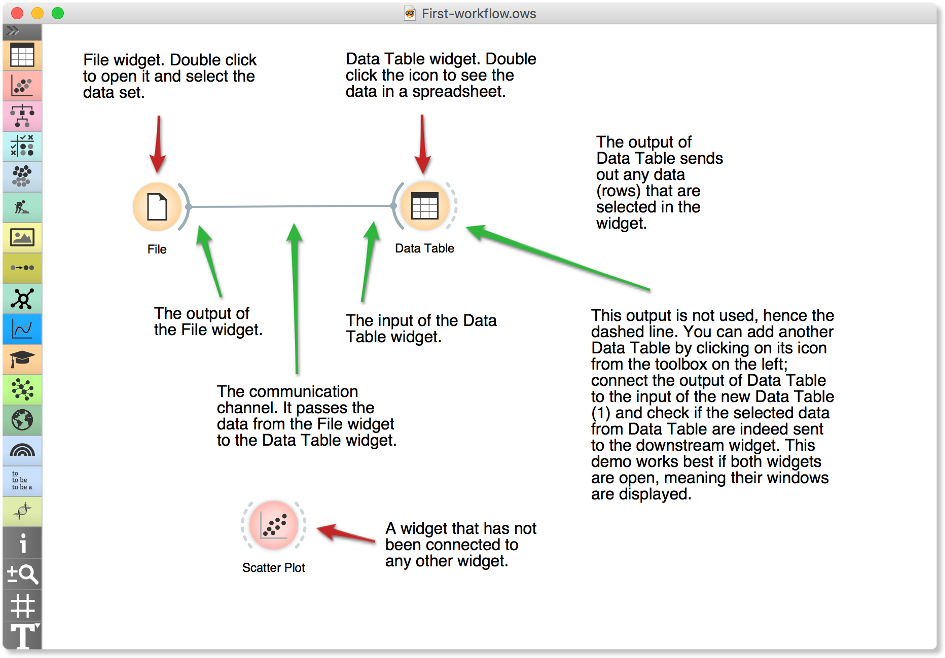
\includegraphics[width=\linewidth]{graphics/ch-workflows/workflow-fig1.png}%
  \caption{A simple workflow with two connected widgets and one widget without connections. The outputs of a widget appear on the right, while the inputs appear on the left.}
  \label{fig:workflow-fig1}
\end{figure*}

We construct workflows by dragging widgets onto the canvas and connecting them by drawing a line from the transmitting widget to the receiving widget. The widget’s outputs are on the right and the inputs on the left. In the workflow above, the File widget sends data to the Data Table widget.
\newpage
Start by constructing a workflow that consists of a File widget, two Scatter Plot widgets and two Data Table widgets:

\begin{figure}[h]
  \centering
  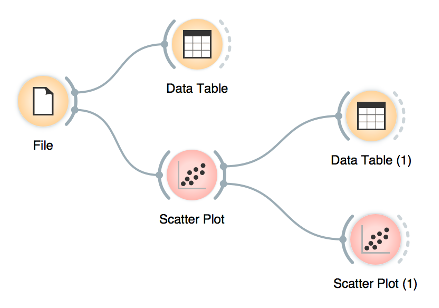
\includegraphics[width=80mm]{graphics/ch-workflows/workflow-fig2.png}%
  \caption{Workflow with a File widget that reads data from disk and sends it to the Scatter Plot and Data Table widget. The Data Table renders the data in a spreadsheet, while the Scatter Plot visualizes it. Selected data points from the plot are sent to two other widgets: Data Table (1) and Scatter Plot (1).}
  \label{fig:workflow-fig2}
\end{figure}

The File widget reads data from your local disk. Open the File widget by double clicking its icon. \mutation\  comes with several pre-loaded data sets. From these (“Browse documentation data sets…”), choose \textit{brown-selected.tab}, a yeast gene expression data set.

\begin{figure}[h]
  \centering
  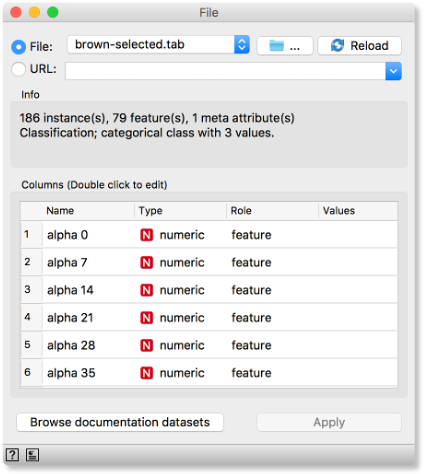
\includegraphics[width=85mm]{graphics/ch-workflows/workflow-fig3.png}%
  \caption{\mutation\  workflows often start with a File widget. The brown-selected data set comprises of a 186 rows (genes) and 81 columns. Out of the 81 columns, 79 contain gene expressions of baker’s yeast under various conditions, one column (marked as a “meta attribute”) provides gene names, and one column contains the “class” value or gene function.}
  \label{fig:workflow-fig3}
\end{figure}

After you load the data, open the other widgets. In the Scatter Plot widget, select a few data points and watch as they appear in widget Data Table (1). Use a combination of two Scatter Plot widgets, where the second scatter plot shows a detail from a smaller region selected in the first scatter plot.

The following is more of a side note, but it won’t hurt. Namely, the scatter plot for a pair of random features does not provide much information on gene function. Does this change with a different choice of feature pairs in the visualization? Rank projections (the button on the top left of the Scatter Plot widget) can help you find a good feature pair. How do you think this works? Could the suggested pairs of features be useful to a biologist?

\begin{figure*}[h]
  \centering
  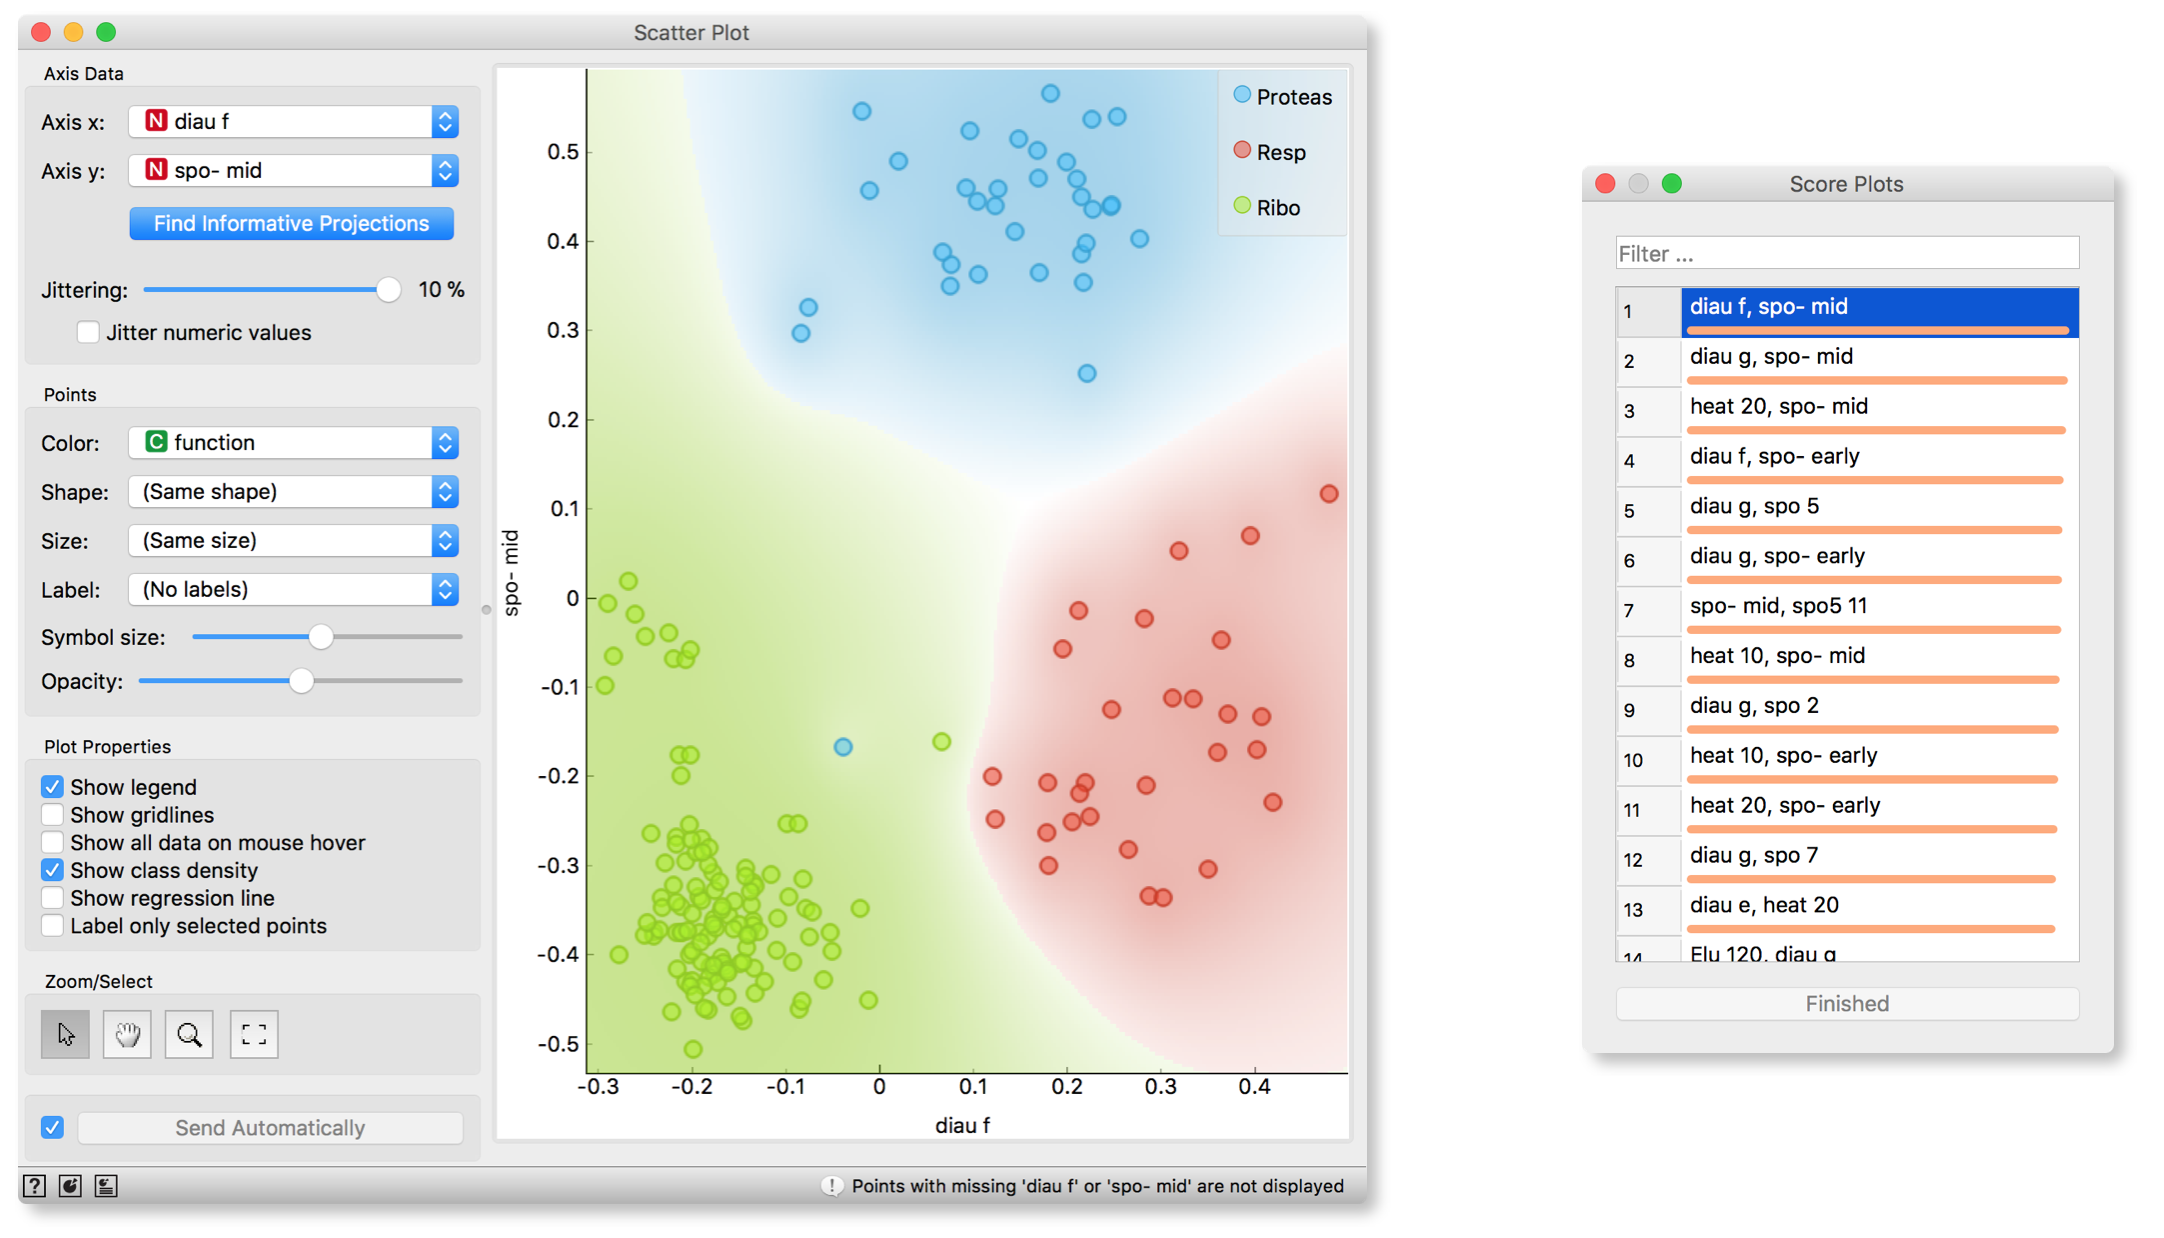
\includegraphics[width=\linewidth]{graphics/ch-workflows/workflow-fig4b.png}
  \caption{Scatter Plot and Ranking}
  \label{fig:workflow-fig4}
\end{figure*}


We can connect the output of the Data Table widget to the Scatter Plot widget to highlight the chosen data instances (rows) in the scatter plot.

\begin{figure}
%   \centering
  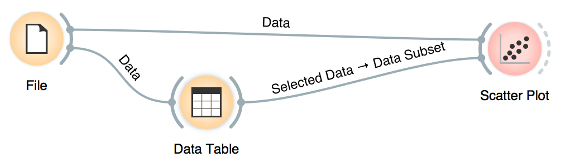
\includegraphics[width=100mm]{graphics/ch-workflows/workflow-fig5.png}
  \caption{In this workflow, we have switched on the option “Show channel names between widgets” in File/Preferences.}
  \label{fig:workflow-fig5}
\end{figure}

How does \mutation\  distinguish between the primary data source and the data selection? It uses the first connected signal as the entire data set and the second one as its subset. To make changes or to check what is happening under the hood, double click on the line connecting the two widgets.
\newpage


\begin{figure*}[h]
%   \centering
  \flushright
  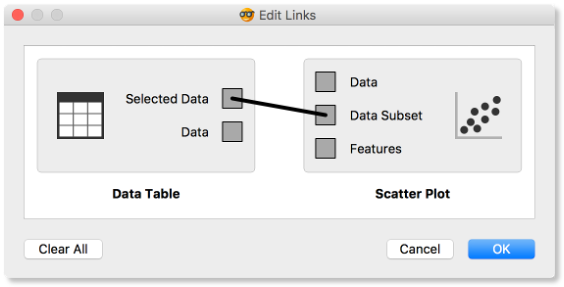
\includegraphics[width=100mm]{graphics/ch-workflows/workflow-fig6.png}
\label{fig:workflow-fig6}%
\end{figure*}

The rows in the data set we are exploring in this lesson are gene profiles. We could perhaps use widgets from the Bioinformatics add-on to get more information on the genes we selected in any of the \mutation\ widgets.

\begin{figure*}[h]
%   \centering
  \flushright
  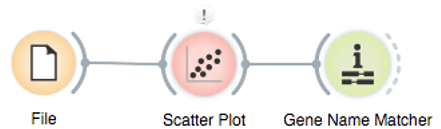
\includegraphics[width=80mm]{graphics/ch-workflows/workflow-fig7.png}%
\label{fig:workflow-fig7}%
\end{figure*}

\marginnote{\textbf{\mutation\ comes with a basic set of widgets for data input, preprocessing, visualization and modeling. For other tasks, like text mining, network analysis, and bioinformatics, there are add-ons. Check them out by selecting Add-ons... from the Options menu.}}
% Lesson 2: Basic Data Exploration
%\chapter{Basic data exploration}
\label{ch:basic_data_exploration}

\newthought{Let us consider another problem} Let us consider another problem, this time from clinical medicine. We will dig for something interesting in the data and explore it a bit with visualization widgets. You will get to know Quasar better, and also learn about several interesting visualizations.

We will start with an empty canvas; to clean it from our previous lesson, use either File/New or select all the widgets and remove them (use the backspace/delete key, or Cmd-backspace if you are on Mac).

Now again, add the File widget and open another documentation data set: heart\_disease. How does the data look like?

\begin{figure}[h]
  \centering
  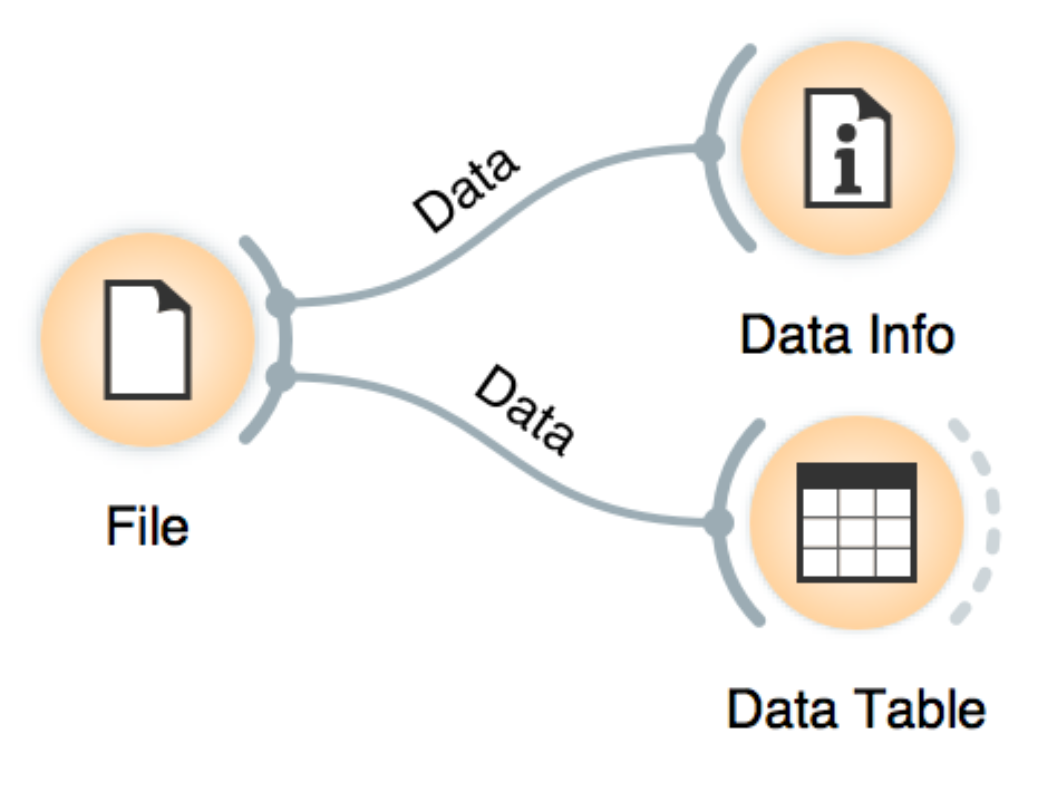
\includegraphics[width=50mm]{graphics/ch-basic_data_exploration/basic_data_exploration-fig1.png}%
  \caption{A simple workflow to inspect the loaded dataset.}
  \label{fig:basic_data_exploration-fig1}
\end{figure}

Let us check whether common visualizations tell us anything interesting. (Hint: look for gender differences. These are always interesting and occasionally even real.)

\begin{figure}[h]
  \centering
  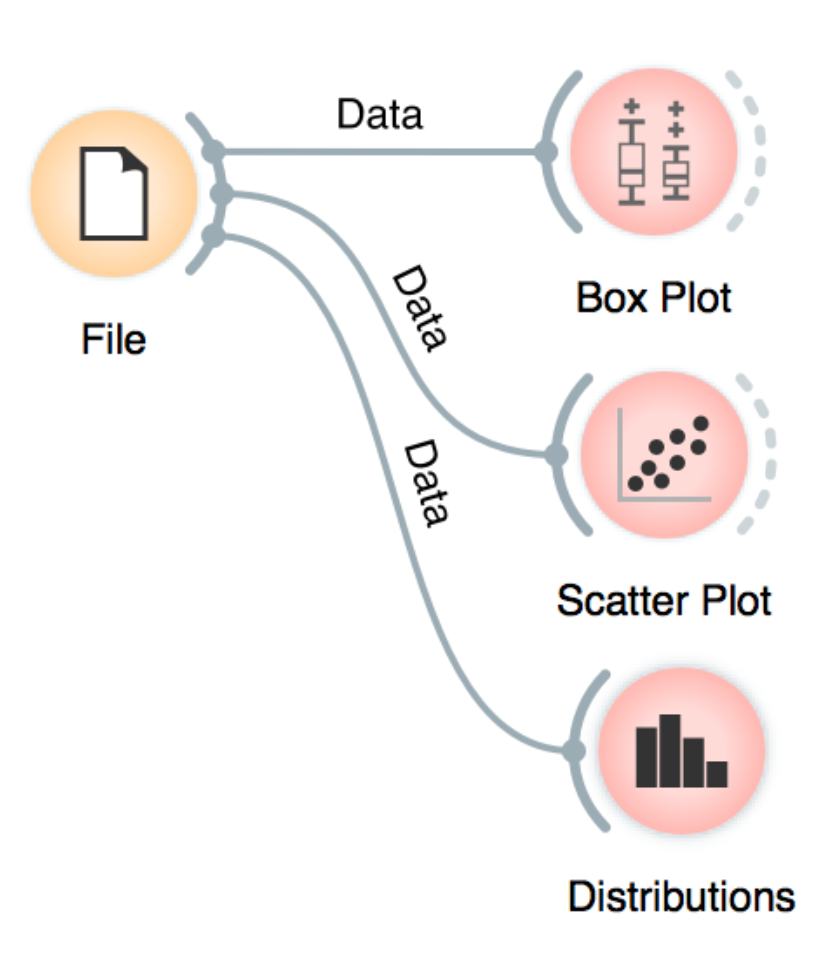
\includegraphics[width=50mm]{graphics/ch-basic_data_exploration/basic_data_exploration-fig2.png}%
  \caption{Quick check with common statistics and other visualization widgets.}
  \label{fig:basic_data_exploration-fig2}
\end{figure}

\newpage
Data can also be split by the value of features—in this case—the gender.

\begin{figure}[h]
  \centering
  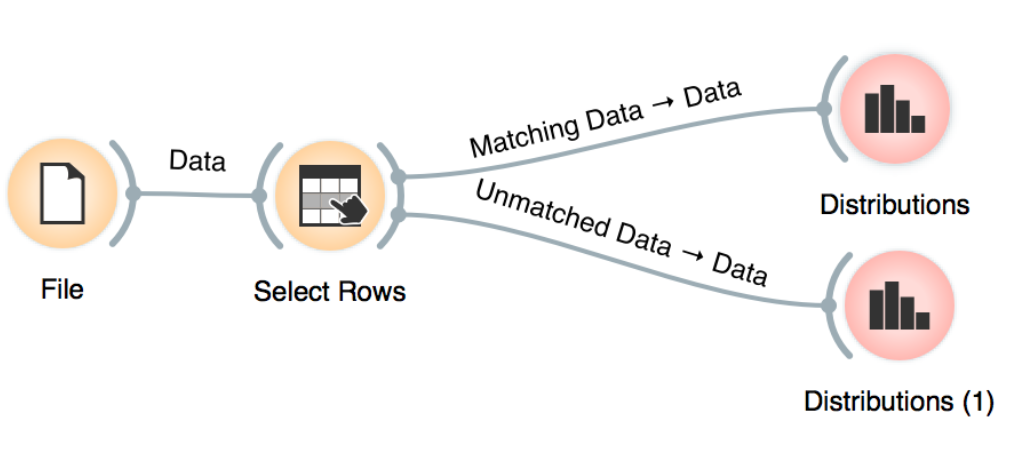
\includegraphics[width=90mm]{graphics/ch-basic_data_exploration/basic_data_exploration-fig3.png}%
  \caption{The two Distributions widgets get different data: the upper gets the selected rows and the lower gets the rest. Double-click the connection between the widgets to access setup dialog, as you've learned in the previous lesson.}
  \label{fig:basic_data_exploration-fig3}
\end{figure}

In the Select Rows widget, we select the female patients. You can also add other conditions. Selection of data instances provides a powerful combination with visualization of data distribution. Try having at least two widgets open at the same time and explore the data.

\begin{marginfigure}
%   \centering
  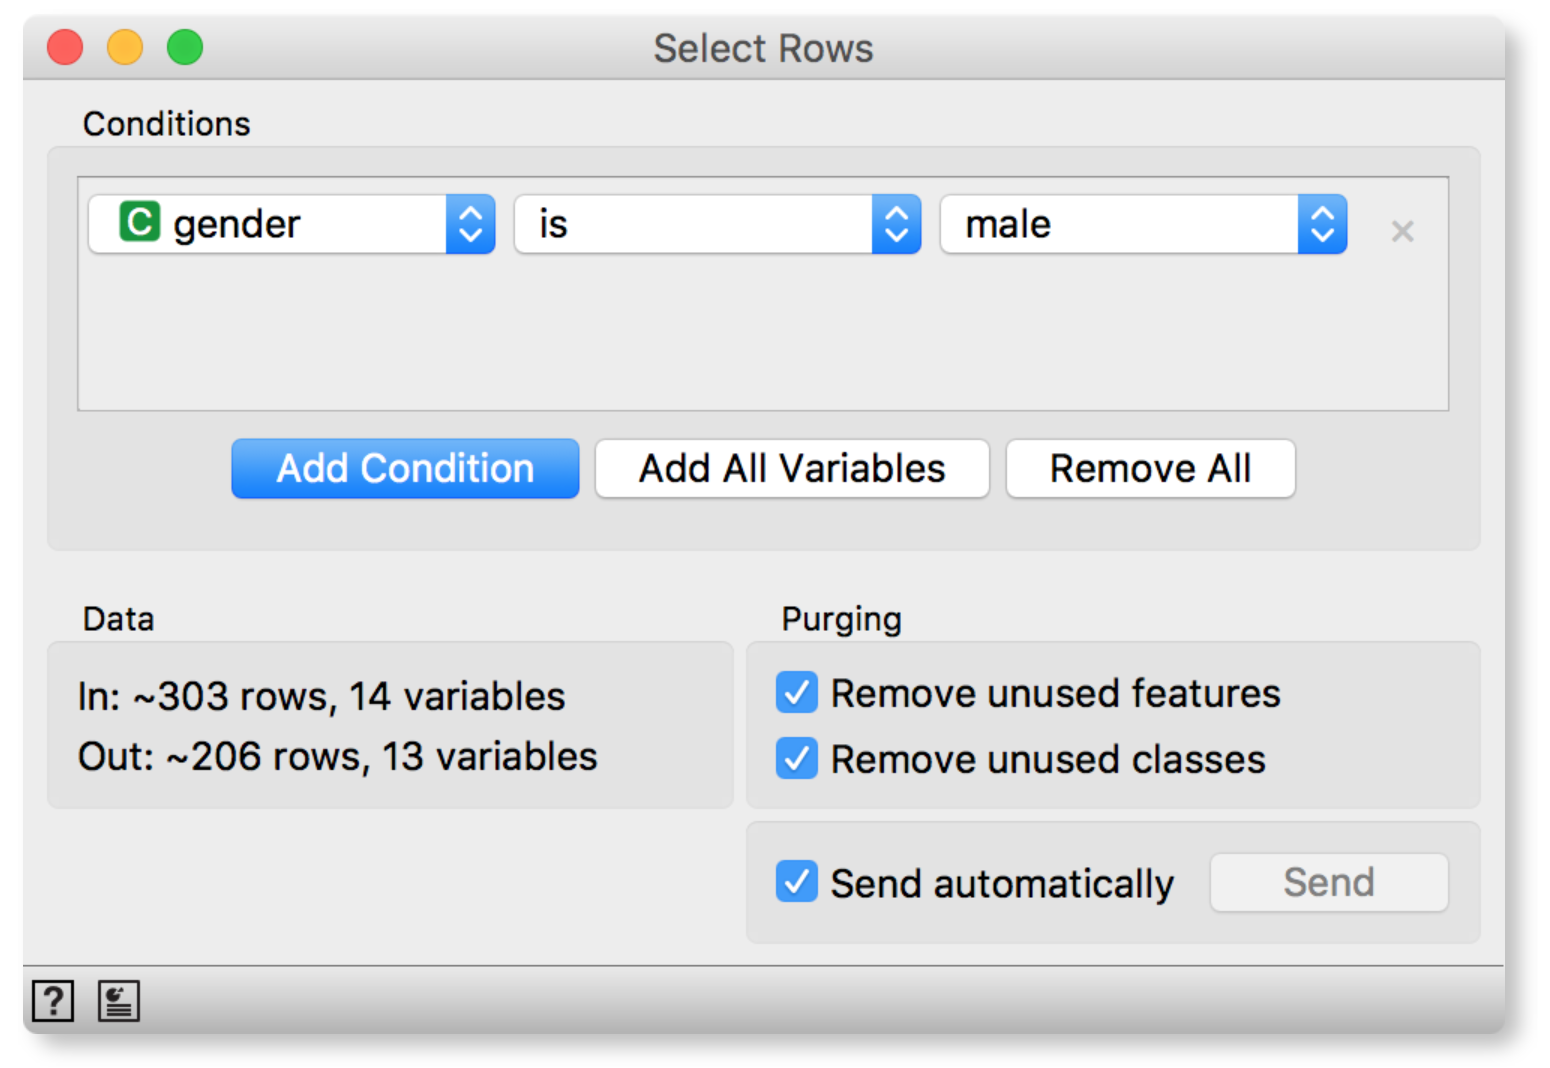
\includegraphics[width=\linewidth]{graphics/ch-basic_data_exploration/basic_data_exploration-fig4.png}%
  \caption{Select Rows and Distributions widget}
  \label{fig:basic_data_exploration-fig4}
\end{marginfigure}

\begin{figure*}[h]
%   \centering
  \flushright
  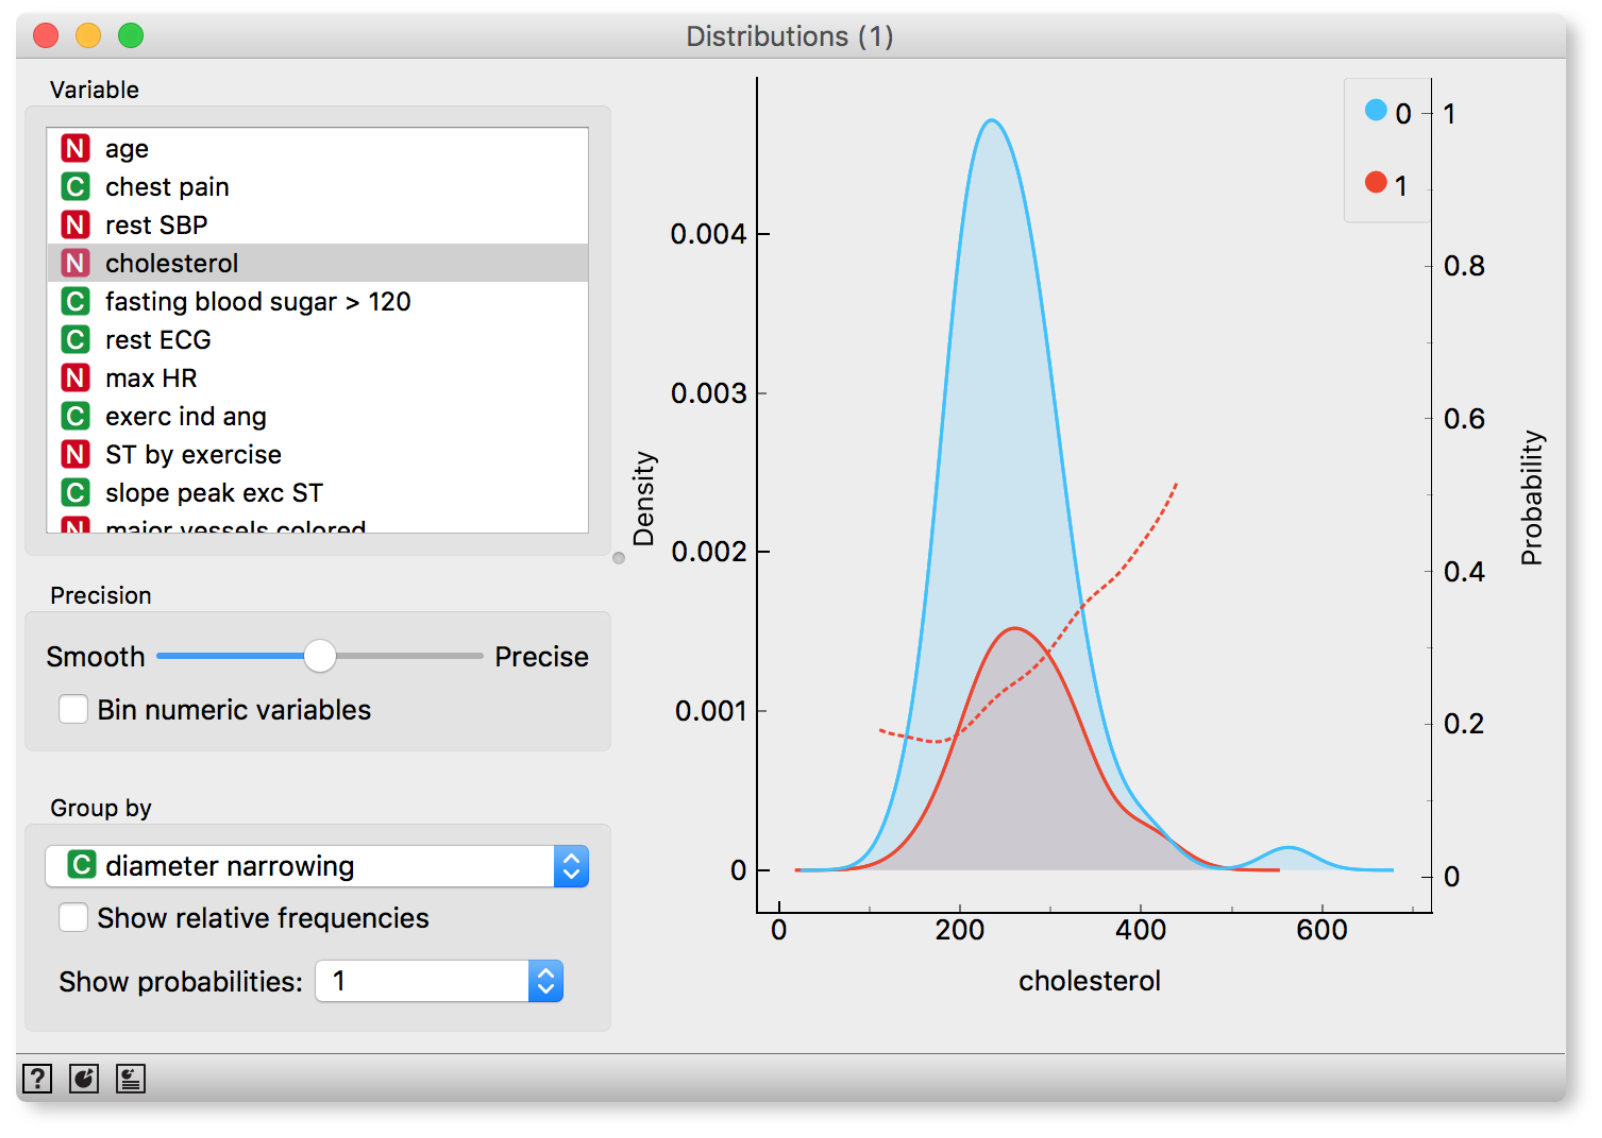
\includegraphics[width=115mm]{graphics/ch-basic_data_exploration/basic_data_exploration-fig5.png}
%   \caption{Scatter Plot and Ranking}
  \label{fig:basic_data_exploration-fig5}
\end{figure*}

There are two less known — but great — visualizations for observing interactions between features. 

Mosaic display shows a rectangle split into columns with widths reflecting the prevalence of different types of chest pain. Each column is then further split vertically according to gender distributions within the column. The resulting rectangles are split again horizontally according to age group sizes. Within the resulting bars, the red and blue areas represent the outcome distribution for each group and the tiny strip to the left of each shows the overall distribution.

\newpage
What can you read from this diagram?

\begin{figure}[h]
  \centering
  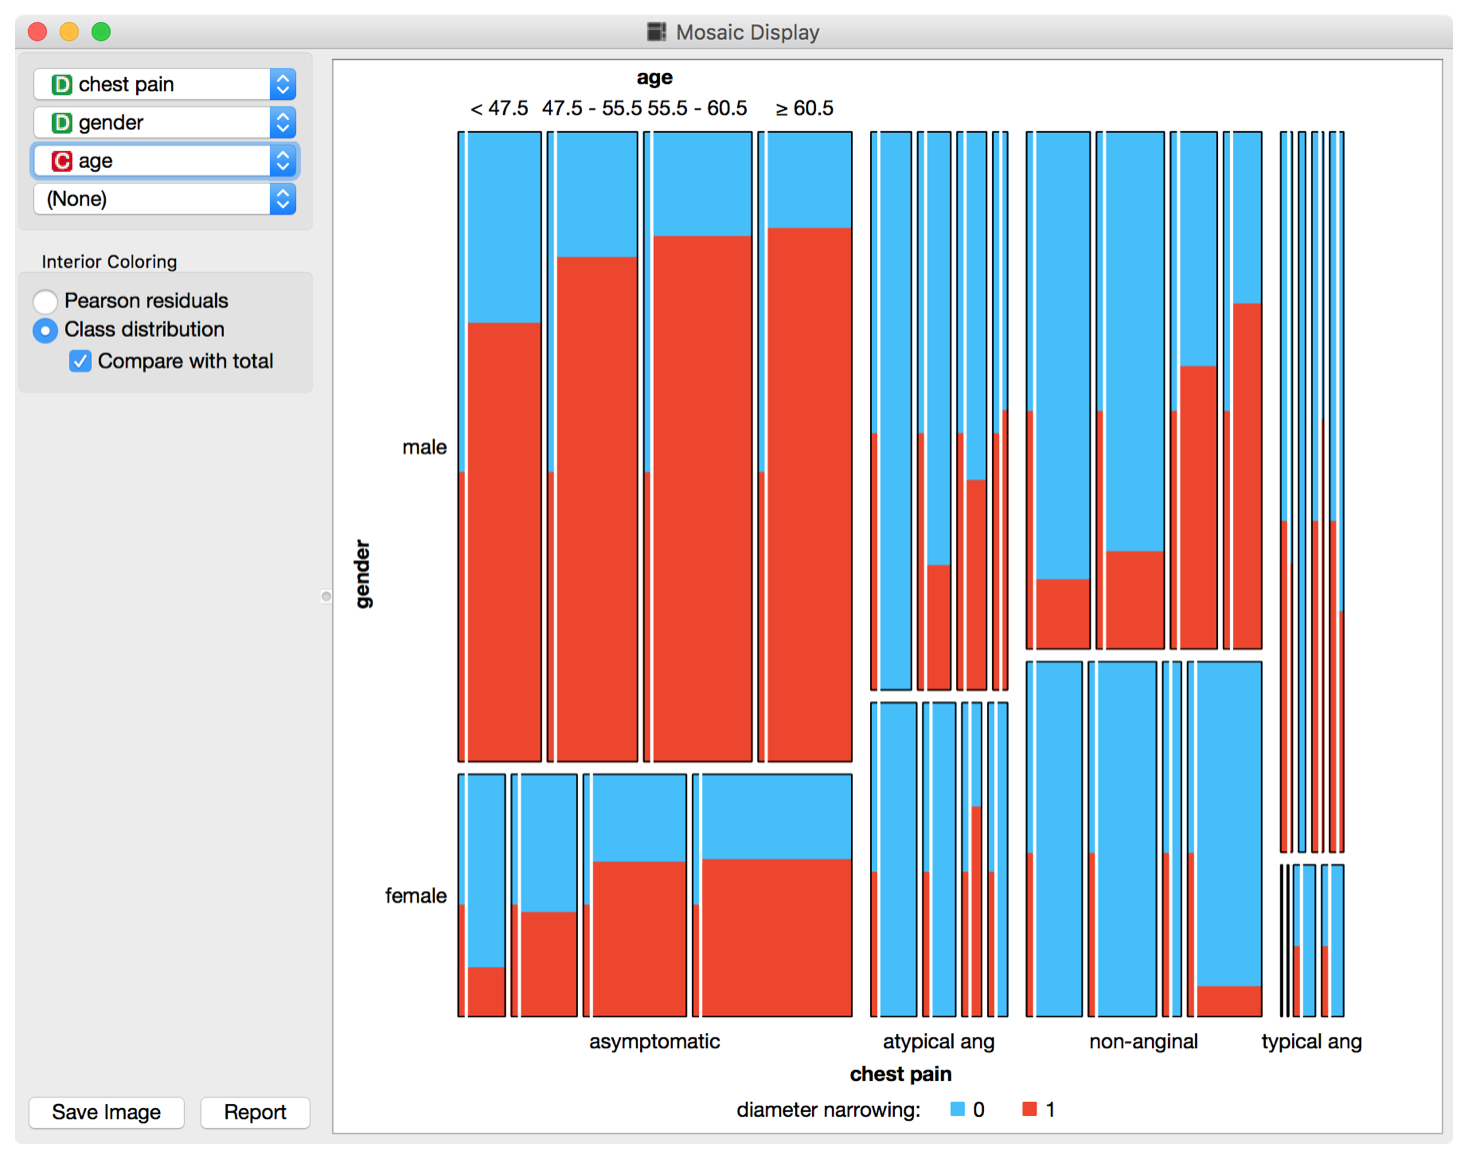
\includegraphics[width=\linewidth]{graphics/ch-basic_data_exploration/basic_data_exploration-fig6.png}
  \caption{You can play with the widget by trying different combinations of 1-4 features.}
  \label{fig:basic_data_exploration-fig6}
\end{figure}

Another visualization, Sieve diagram also splits a rectangle horizontally and vertically, but with independent cuts, so the areas correspond to the expected number of data instances if the observed variables were independent. For instance, 1/4 of patients are older than 60, and 1/3 of patients are female, so the area of the bottom right rectangle is 1/12 of the total area. With roughly 300 patients, we would expect 1/12 × 300 = 25 older women in our data. As a matter of fact, there are 34. Sieve diagram shows the difference between the expected and the observed frequencies by the grid density and the color of the field.

\begin{figure}
  \flushright
  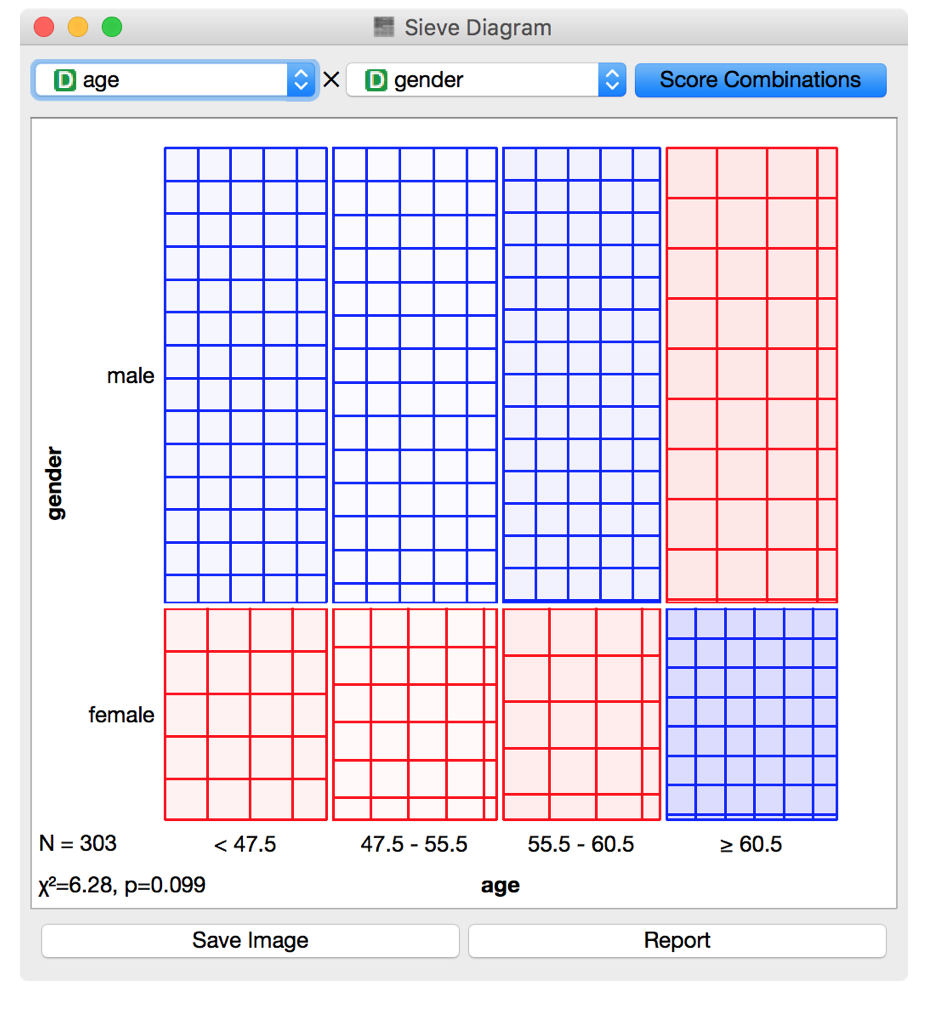
\includegraphics[width=70mm]{graphics/ch-basic_data_exploration/basic_data_exploration-fig7.png}
  \caption{See the Score Combinations button? Guess what it does? And how it scores the combinations? (Hint: there are some Greek letters at the bottom of the widget.)}
  \label{fig:basic_data_exploration-fig7}
\end{figure}
% Lesson 3: Saving Your Work
%\chapter{Saving your work}
\label{ch:saving_your_work}

\newthought{At the end of a lesson}, your workflow may look like this:
\begin{figure}[h]
  \centering
  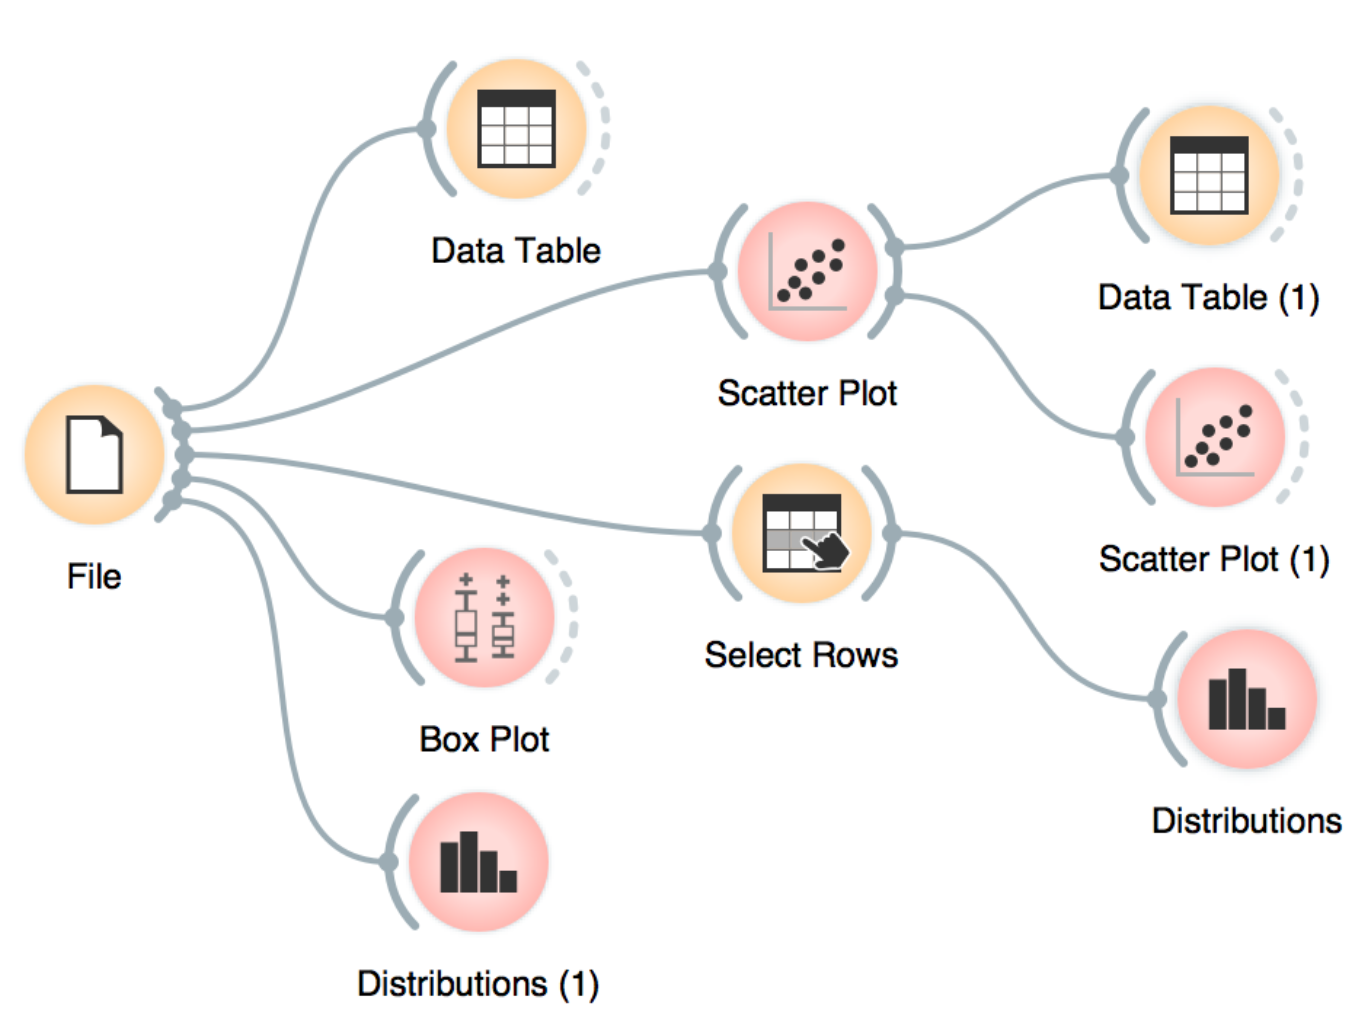
\includegraphics[width=65mm]{graphics/ch-saving/saving-fig1.png}%
  \caption{A fairly complex workflow that you would want to share or reuse at a later time.}
  \label{fig:saveing-fig1}
\end{figure}

You can save this processing workflow, otherwise called "\textit{Schema}" using the File/Save menu and share it with your colleagues. Just don't forget to put the data files in the same directory as the file with the workflow.

Widgets also have a Report button in their bottom status bar, which you can use to keep a log of your analysis. When you find something interesting, just click it and the graph \marginnote{Clicking on a section of the report window allows you to add a comment.} will be added to your log. You can also add reports from the widgets on the path to this one, to make sure you don't forget anything relevant.

\begin{marginfigure}
%   ~\vspace{0.5cm}
  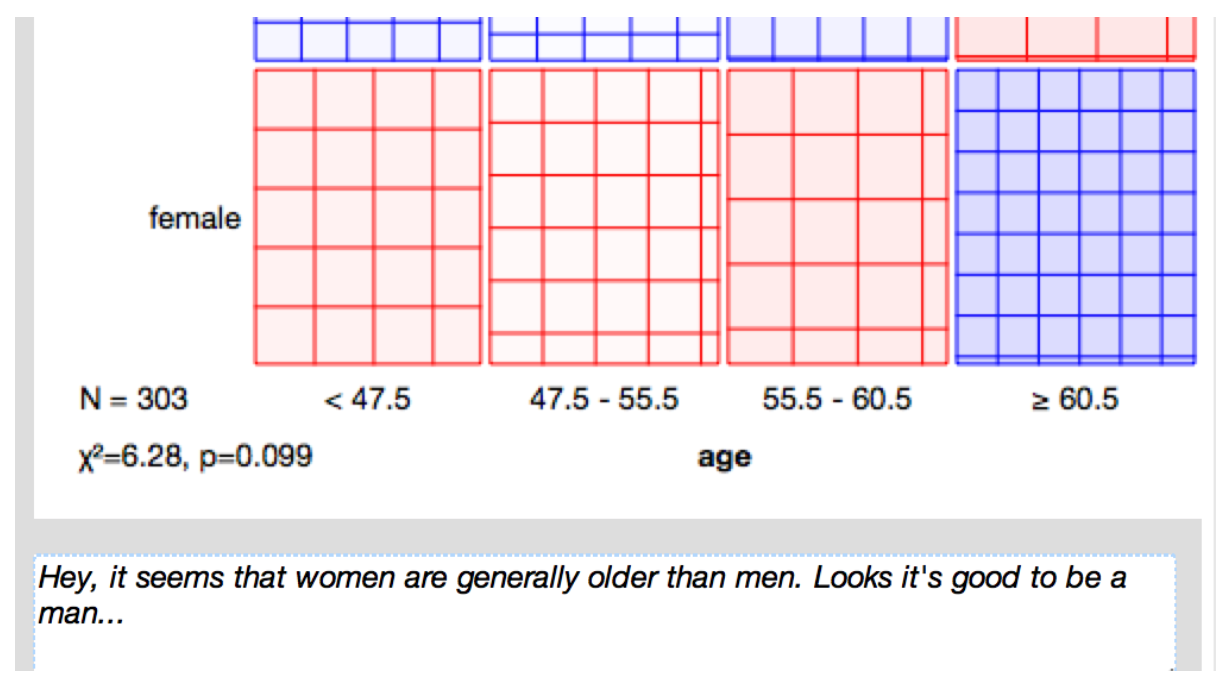
\includegraphics[width=60mm]{graphics/ch-saving/saving-fig3.png}%
  ~\vspace{1.0cm}
  \caption{The report window (left) and the additional text input box (top).}
  \label{fig:saveing-fig3}
\end{marginfigure}

\begin{figure}[h]
  \centering
  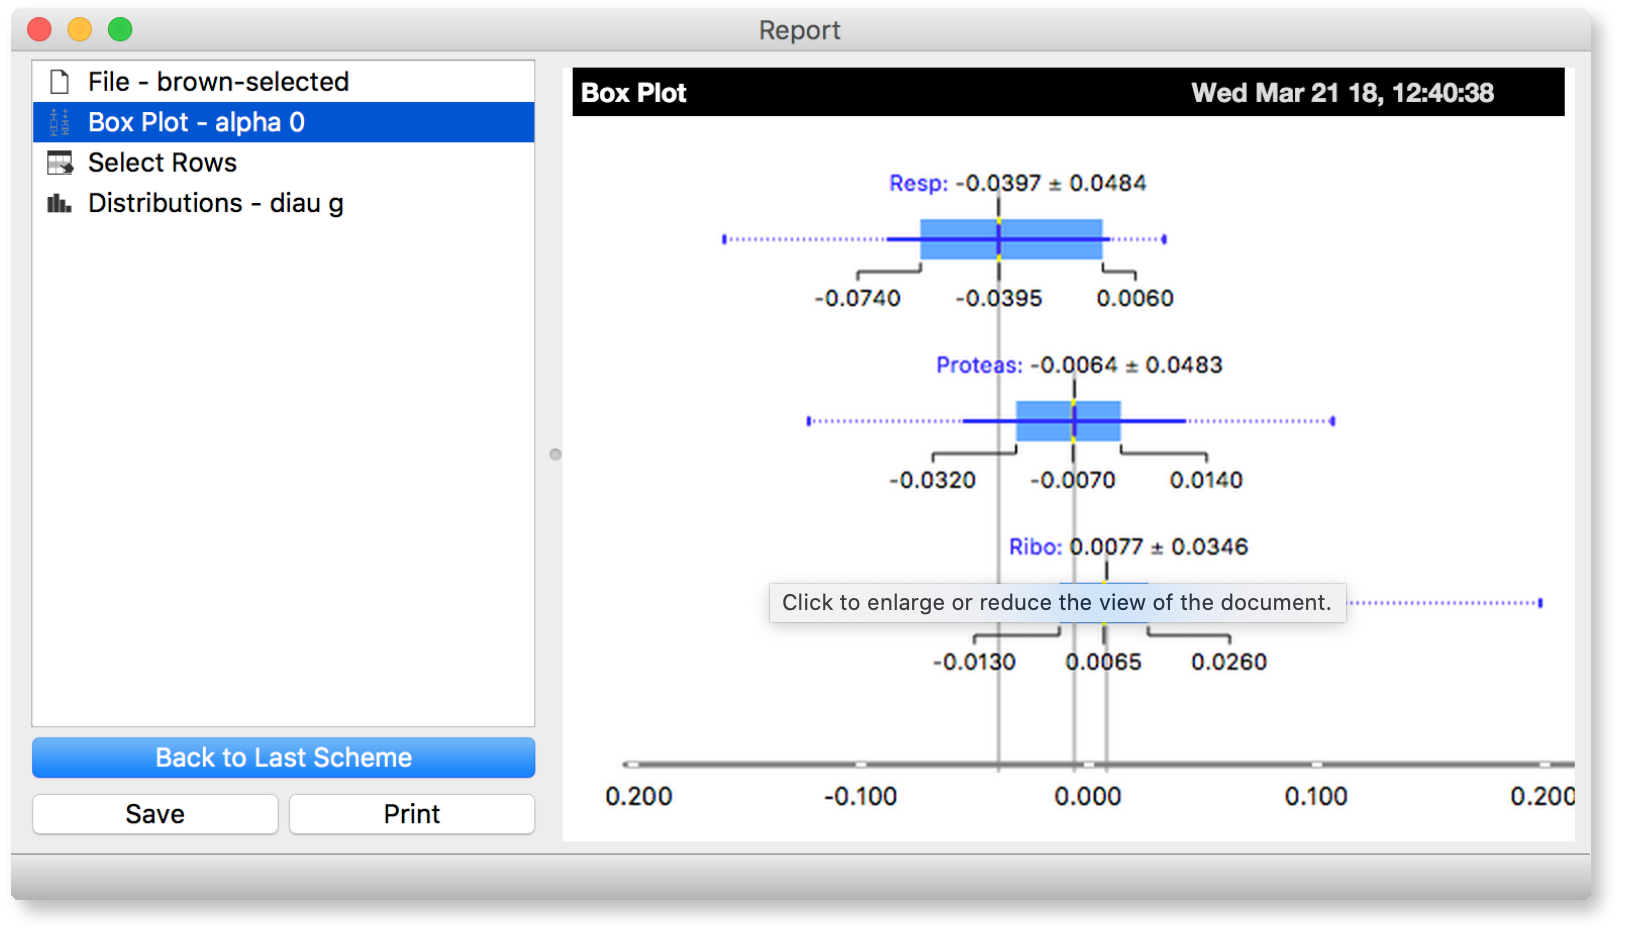
\includegraphics[width=90mm]{graphics/ch-saving/saving-fig2.png}%
  \label{fig:saveing-fig2}
\end{figure}

You can save the report as HTML or PDF, or a report file that includes all workflow related report items that you can later open in Orange. In this way, you and your colleagues can reproduce your analysis results.
% Lesson 4: Loading Your Own Data Set
%\chapter{Loading data sets}
\label{ch:loading_data}

\newthought{The data sets we have worked with} in the previous lesson come with the \mutation\ installation. \mutation\ can read data from many file formats which include tab and comma separated and Excel files. To see how this works, let's prepare a data set (with school subjects and grades) in Excel and save it on a local disk.

\begin{figure}[h]
  \centering
  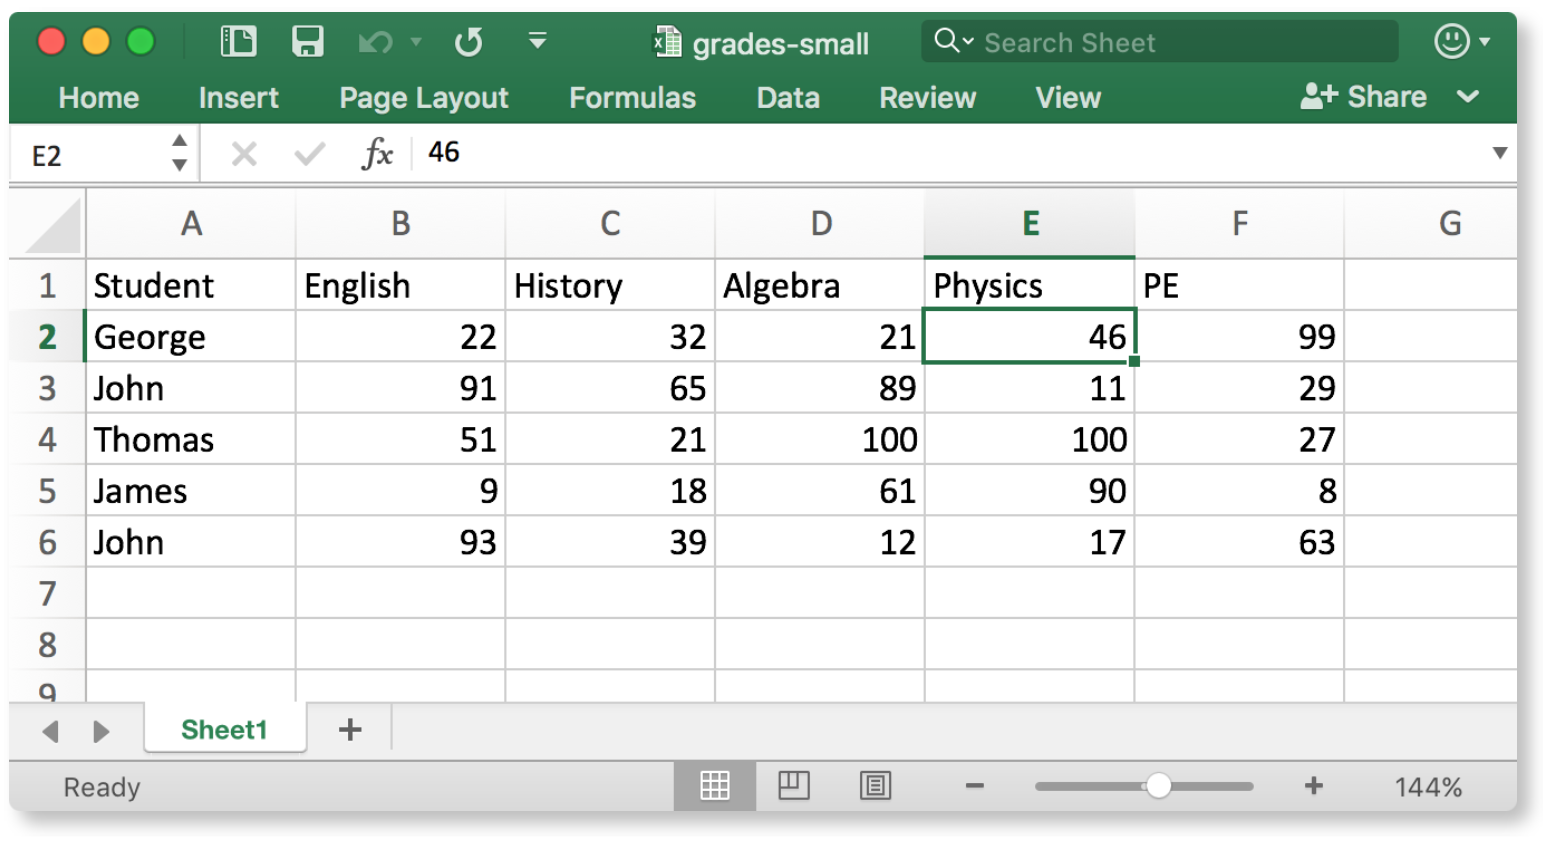
\includegraphics[width=90mm]{graphics/ch-loading_data/loading-fig1.png}%
  \caption{Make a spreadsheet in Excel with the numbers shown on the left. Of course, you can use any other editor, but remember to save your file in the \textit{comma separated values} (*.csv) format.}
  \label{fig:loading-fig1}
\end{figure}

In \mutation, we can use, for example, the File widget to load this data set.

\begin{figure}[h]
  \centering
  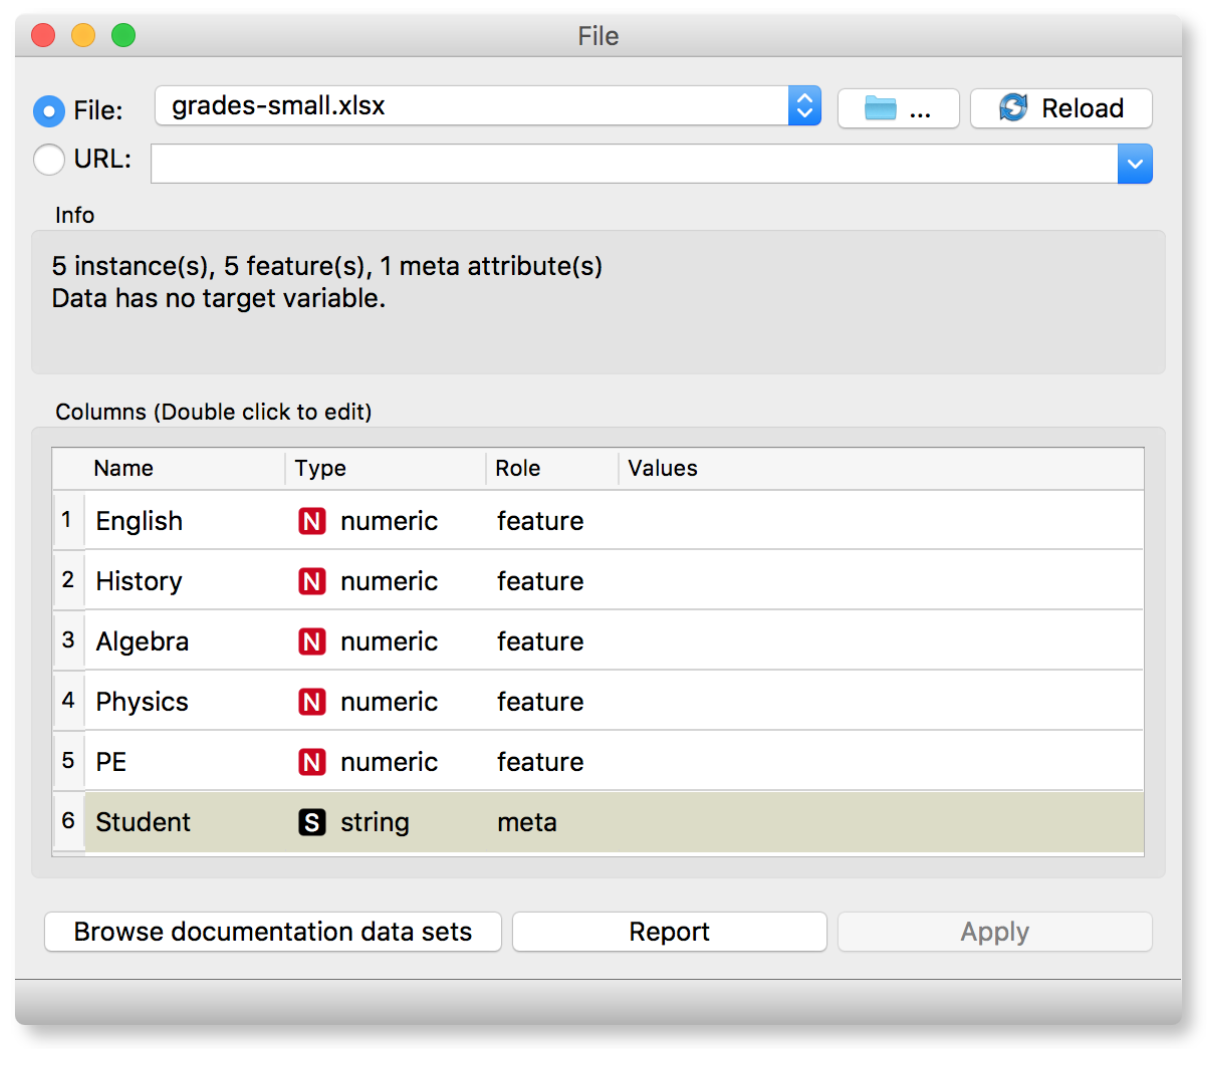
\includegraphics[width=90mm]{graphics/ch-loading_data/loading-fig2.png}%
  \caption{The \textit{File} widget allows you to select a local file or even paste a URL to a Google Spreadsheet. In the Info box, you will see a quick summary about the data you loaded. By double clicking the fields, you can also edit the types of entries and their role, that will be relevant for further processing.}
  \label{fig:loading-fig2}
\end{figure}

Looks good! \mutation\ has correctly guessed that student names are character strings and that this column in the data set is special, meant to provide additional information and not to be used for any kind of modeling (more about this in the upcoming lectures). All other columns are numeric features.

It is always good to check if all the data was read correctly. Now, you can connect the \textit{File} widget with the \textit{Data Table} widget,

\begin{figure}[h]
  \centering
  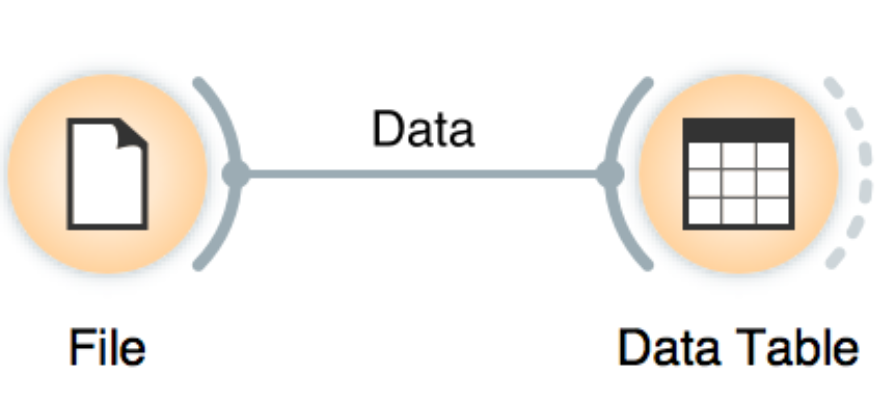
\includegraphics[width=40mm]{graphics/ch-loading_data/loading-fig3.png}%
  \caption{Make the simple workflow shown on the right.}
\label{fig:loading-fig3}
\end{figure}

\noindent and double click on the Data Table to see the data in a spreadsheet format.
Nice, everything is here. 

\begin{figure*}[h]
  \centering
  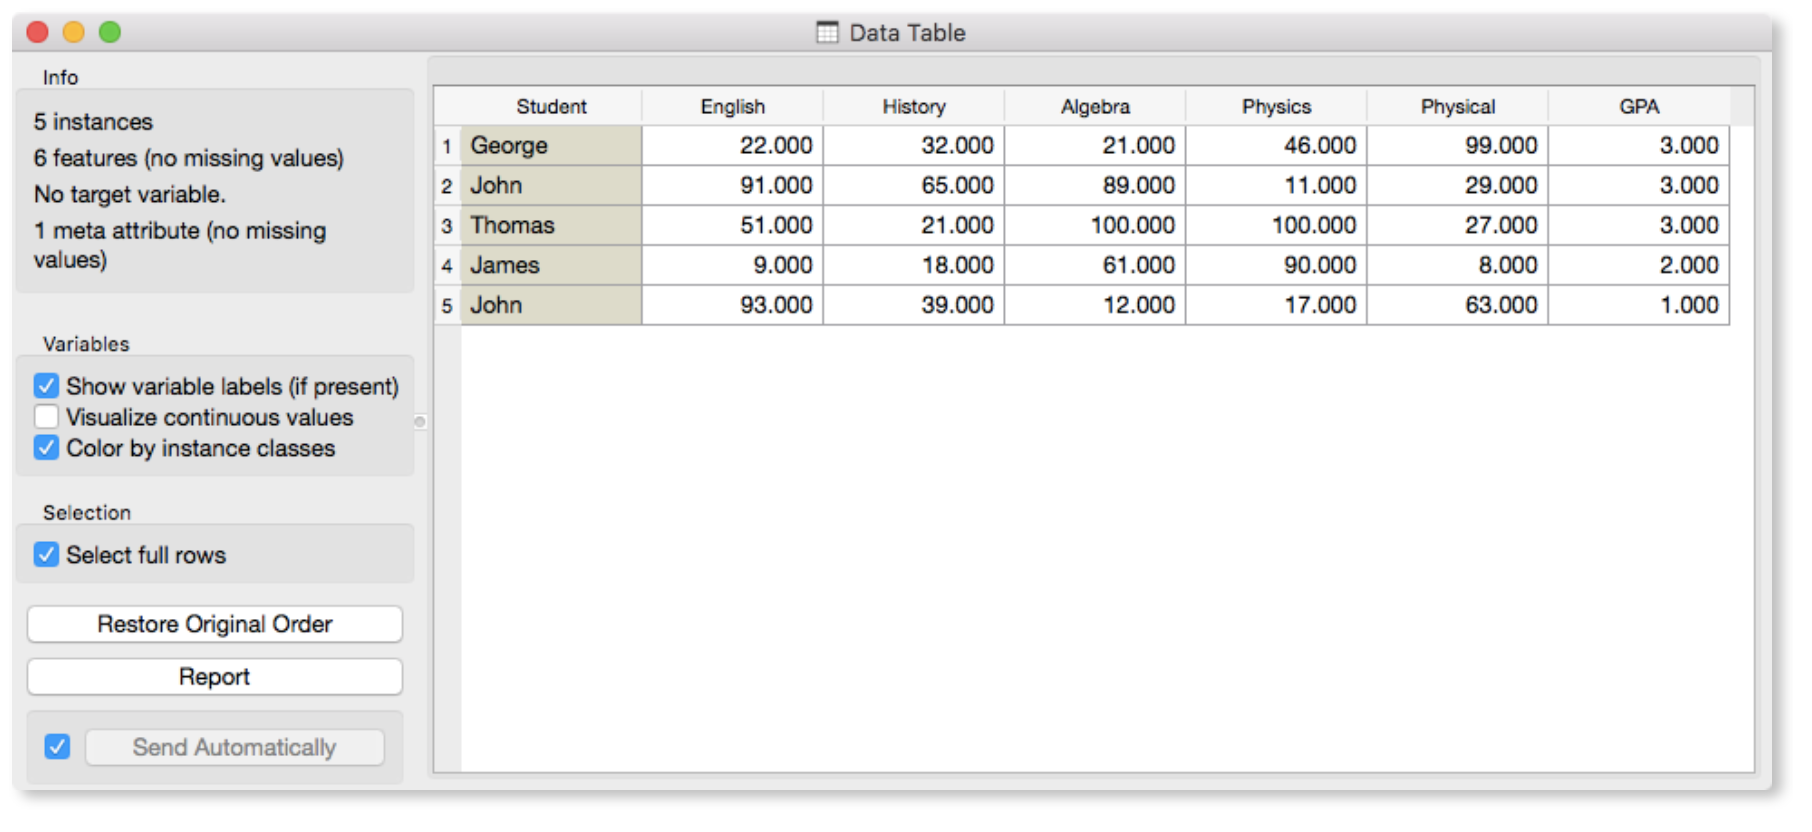
\includegraphics[width=\linewidth]{graphics/ch-loading_data/loading-fig4.png}%
  \caption{The \textit{Data Table} widget shows the loaded data set, you can select rows, which will appear on the output of the widget. It is also possible to do simple data visualizations. Explore the functionalities!}
  \label{fig:loading-fig4}
\end{figure*}

Instead of using Excel, we could also use Google Sheets, a free on-line spreadsheet alternative. Then, instead of finding the file on the local disk, we would enter its URL address to the File widget URL entry box.

\mutation’s legacy native data format is a tab-delimited text file with three header rows. The first row lists the attribute names, the second row defines their type (continuous, discrete, time and string, or abbreviated c, d, t, and s), and the third row an optional role (class, meta, weight, or ignore).

There is more to input data formatting and loading. If you would really like to dive in for more, check out the documentation page on \href{https://orange-visual-programming.readthedocs.io/loading-your-data/index.html}{Loading your Data}, or a \href{https://www.youtube.com/watch?v=MHcGdQeYCMg}{video tutorial} on this subject.

% Lesson 5: Spectral Data
%\chapter{Spectral data}
\label{ch:spectral-data}

\begin{marginfigure}
%   \centering
  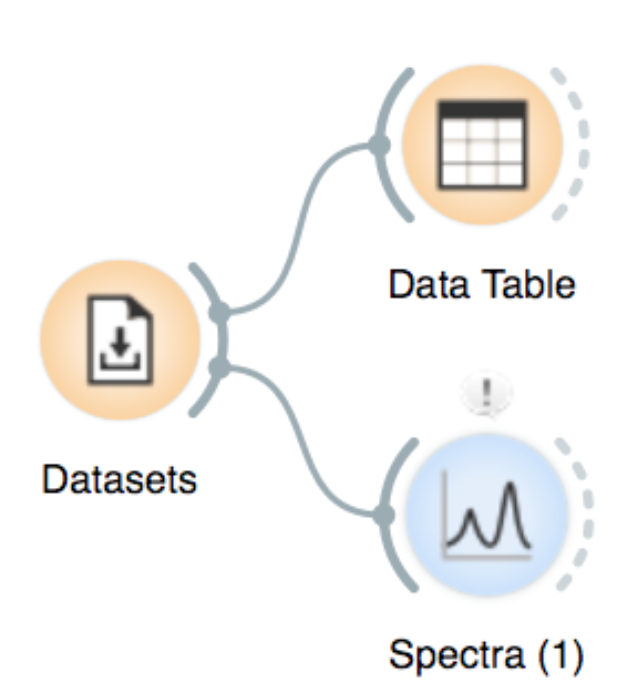
\includegraphics[width=40mm]{graphics/ch-spectral_data/spectral-data-fig1.png}%
  \caption{Your first spectroscopy workflow!}
  \label{fig:spectral-data-fig1}
\end{marginfigure}

\newthought{Let's make the small workflow} shown on the right and open the “Liver spectroscopy” data set from \mutation’s \textit{Datasets} widget.
In a \textit{Data Table}, each row represents a spectrum. For the liver dataset, all columns, except the class column, describe absorbance at a specific wavenumber. Their column names must be numbers, otherwise \mutation’s spectral tools will just enumerate them, starting from 0.

\begin{figure}[h]
  \centering
  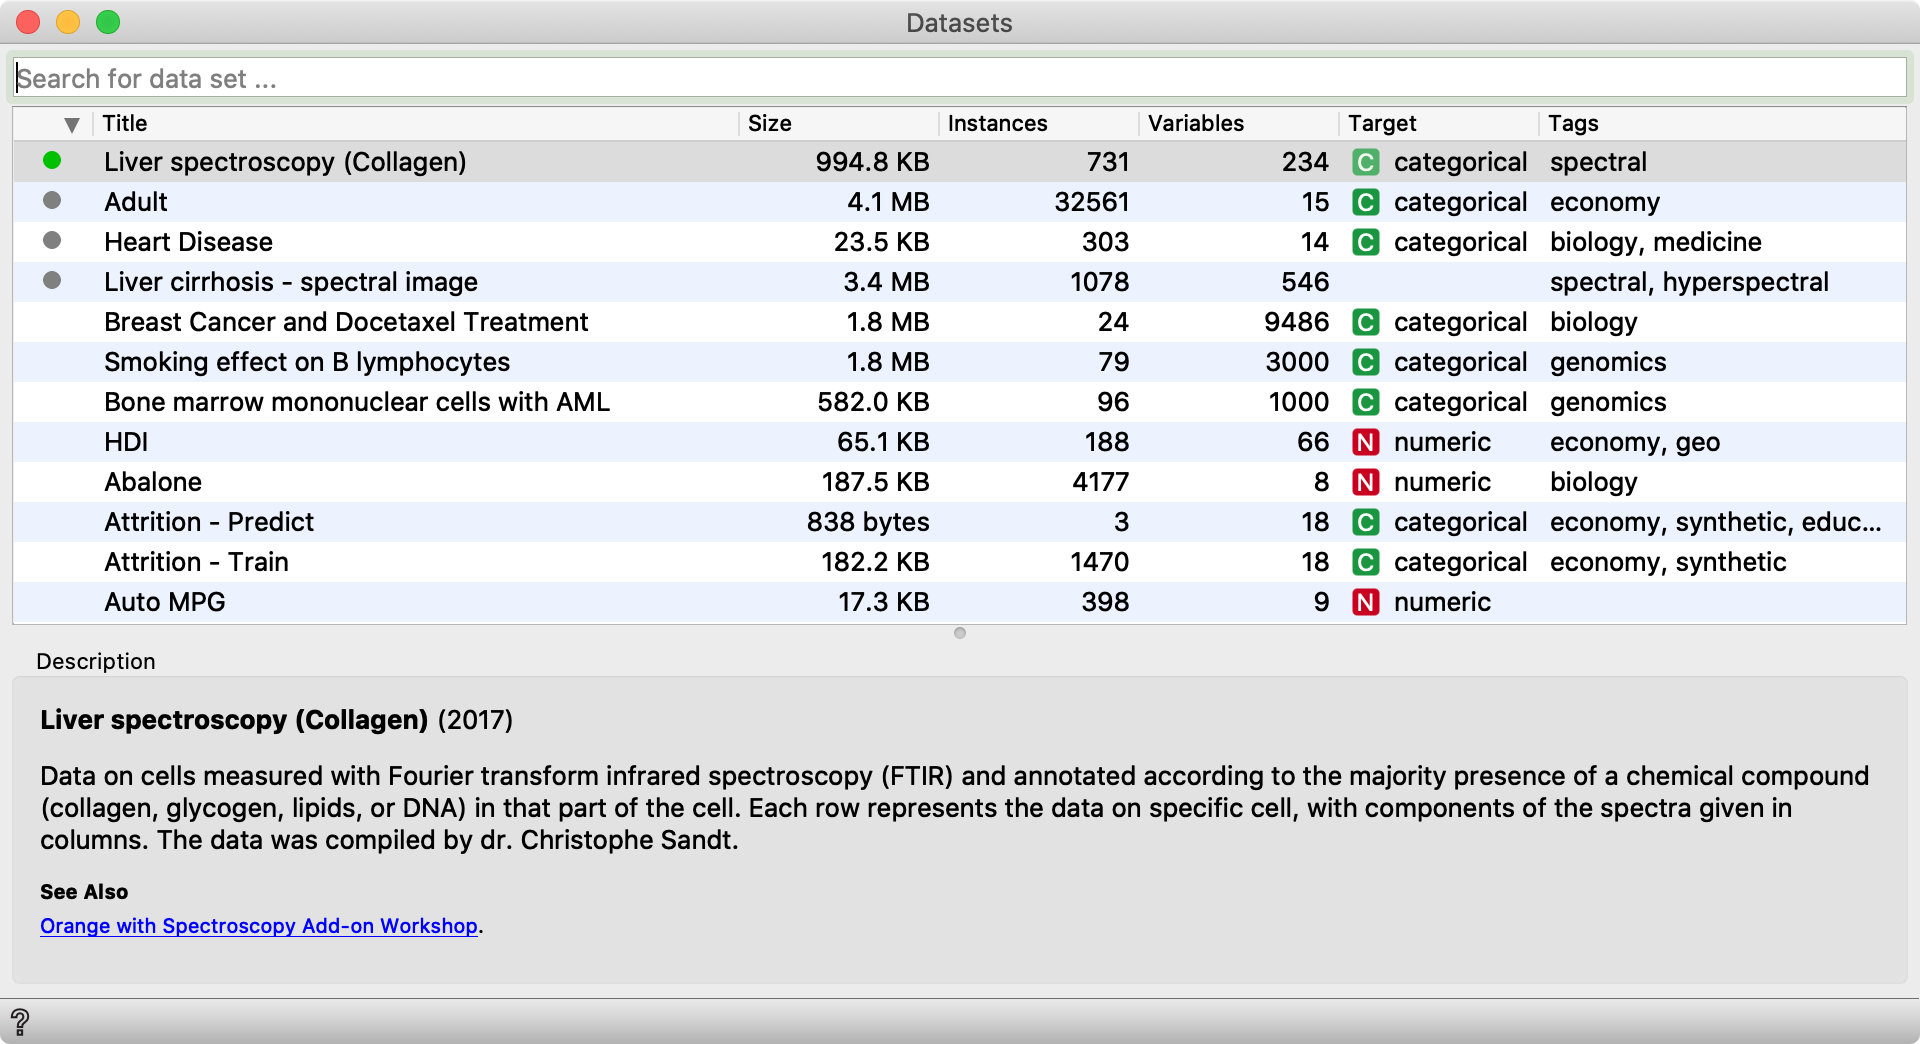
\includegraphics[width=\linewidth]{graphics/ch-spectral_data/spectral-data-fig2.png}%
%   ~\vspace{2cm}
  \caption{The \textit{Datasets} widget provides data for training and testing purposes. The files are stored on a server and to use it, you need a working internet connection, but after you accessed them, they are stored on your computer for off-line use.}
  \label{fig:spectral-data-fig2}
\end{figure}

Connect the data to a \textit{Spectra} widget from the \textbf{Spectroscopy} toolbox. To see the graph below, choose the feature for coloring in the top-left Menu (or click on the graph and press “c”).

\begin{marginfigure}
  \centering
  
\includegraphics[height=55mm]{graphics/fig-spacer.png}\\
  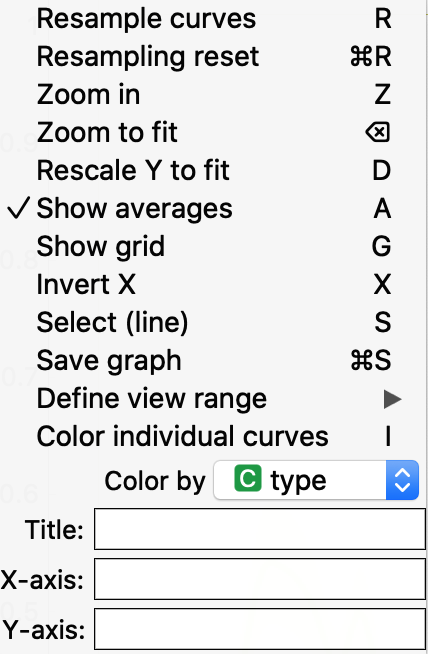
\includegraphics[width=35mm]{graphics/ch-spectral_data/spectral-data-fig4.png}%
  ~\vspace{0.5 cm}
  \caption{The \textit{Spectra} widget and it's options. Try to use keyboard shortcuts on the right for frequent actions.}
  \label{fig:spectral-data-fig4}
\end{marginfigure}

\begin{figure}[h]
  \centering
  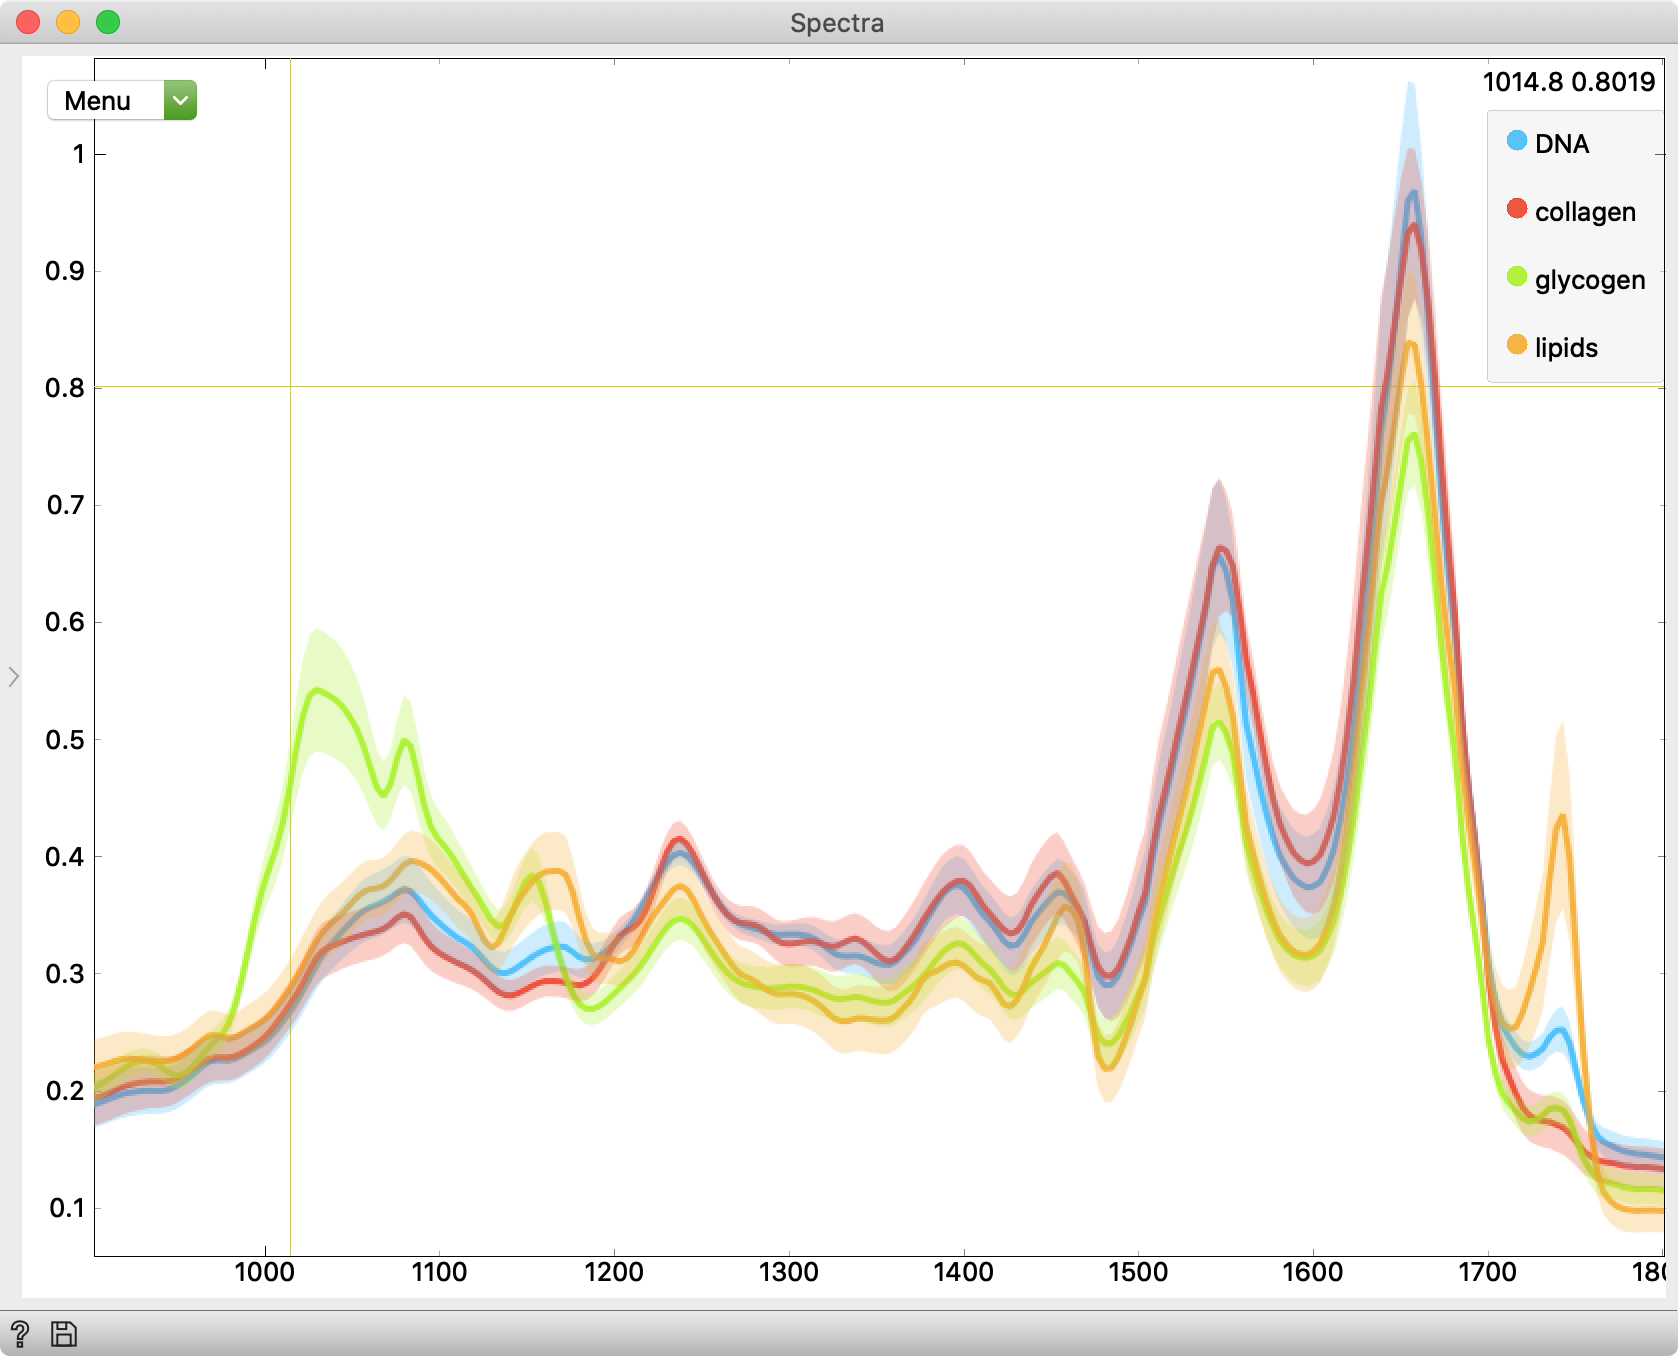
\includegraphics[width=80mm]{graphics/ch-spectral_data/spectral-data-fig3.png}%

  \label{fig:spectral-data-fig3}
\end{figure}

% Lesson 6: PCA on Spectral Data
%\chapter{PCA on spectral data}
\label{ch:spectral-PCA}



\begin{wrapfigure}{o}{0.5\textwidth}
    \centering
    \vspace{-2cm}
    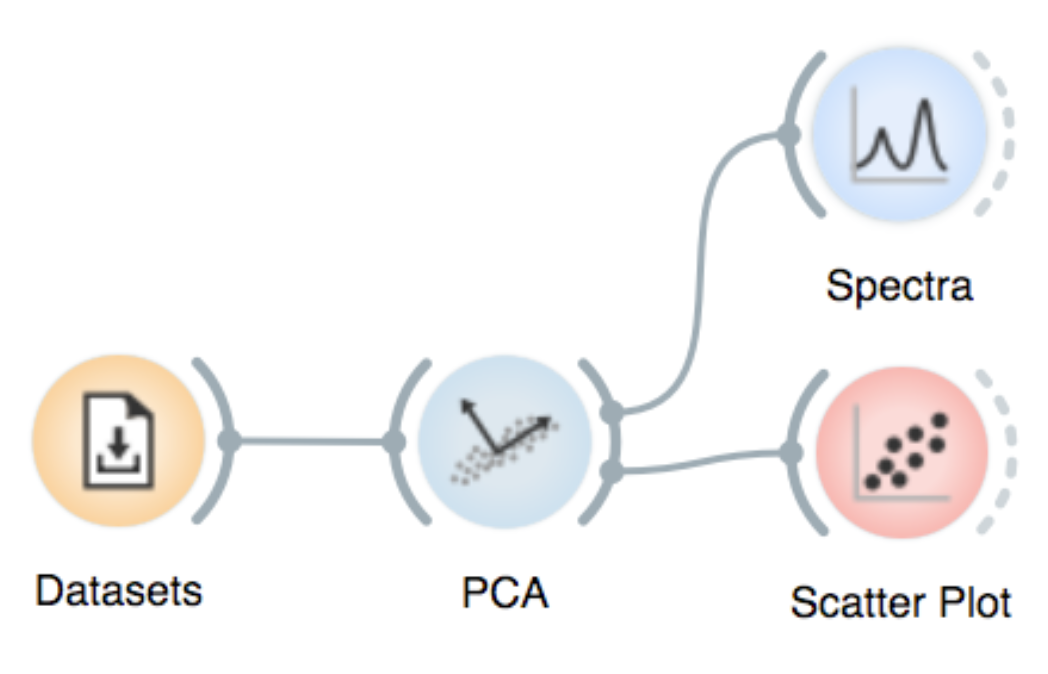
\includegraphics[width=0.55\textwidth]{graphics/ch-spectral_PCA/spectral_PCA-fig1.png}
\end{wrapfigure}

In this lesson we will explore the capabilities of \mutation\ for principal component analysis (PCA) on spectroscopy data. As usual, we will use the Liver Spectroscopy dataset. Connect \textit{Datasets} to the \textit{PCA} widget, choose the first 5 principal components and then connect \textit{PCA’s} default output, "Transformed Data", into the \textit{Scatter Plot}. 

We see that the first two principal components separate majority compounds in that part of the tissue well. 


\begin{figure}[h]
\hspace{-1cm}\stackinset{r}{-0.4\linewidth}{t}{+0.1\linewidth}
  {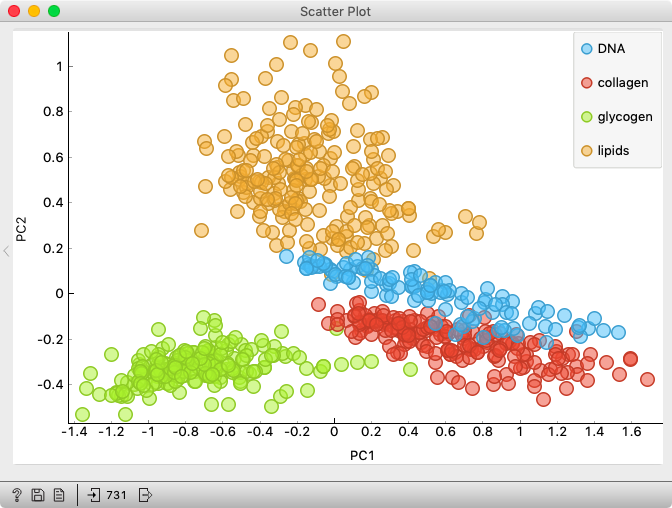
\includegraphics[scale=0.4]{graphics/ch-spectral_PCA/scatterplot.png}}
  {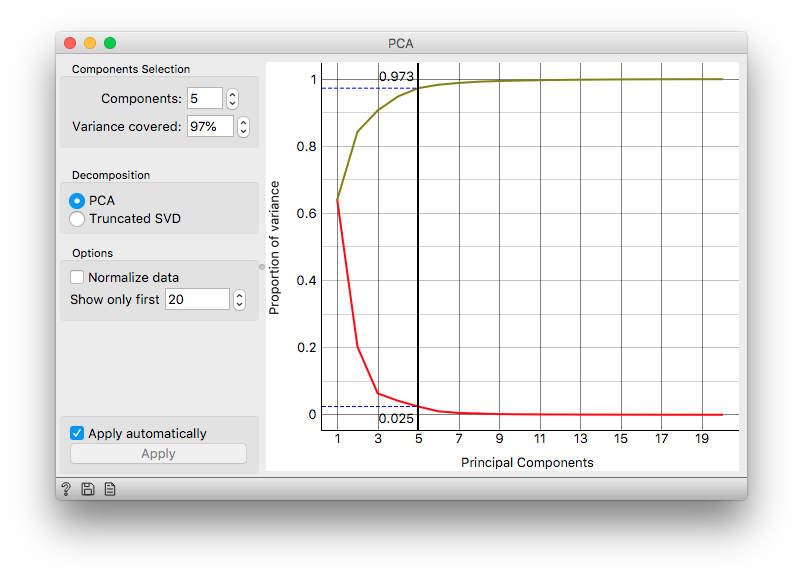
\includegraphics[scale=0.4]{graphics/ch-spectral_PCA/pca.png}}
  \caption{We chose not to normalize variables in \textit{PCA}. Why?}
  \label{fig:spectral-PCA-fig2}
\end{figure}

\begin{wrapfigure}{o}{0.8\textwidth}
  \centering
  \vspace{-0.5cm}
  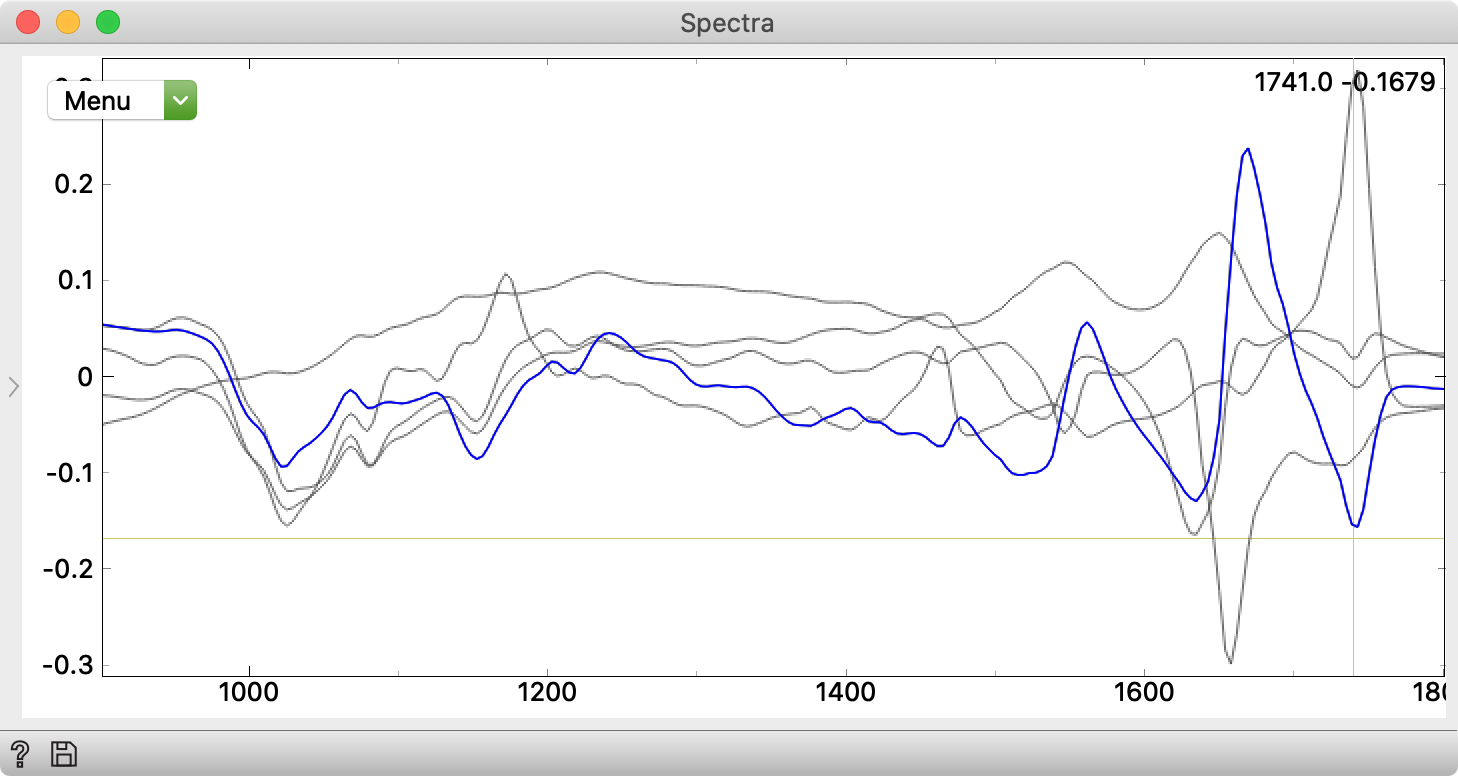
\includegraphics[width=0.8\textwidth]{graphics/ch-spectral_PCA/spectral_PCA-fig3.png}%
  \caption{The curve under the cursor is highlighted. A tooltip will appear after some time. If clicked, the curve will be selected.}
  \label{fig:spectral-PCA-fig3}
\end{wrapfigure}

To see what different principal components represent, connect \textit{PCA’s} "Components" output (be careful, \textit{PCA} has 3 outputs) into \textit{Spectra}. Wondering which principal component is highlighted in the following screenshot? Wait for the tooltip...

Let's extend our workflow. In the next example, we are also using the “Data Subset” input. The \textit{Scatter Plot} and \textit{Spectra (2)} widgets on the right get both the whole data and a subset of it.

\begin{wrapfigure}{o}{0.7\textwidth}
  \centering
%   \vspace{-2cm}
  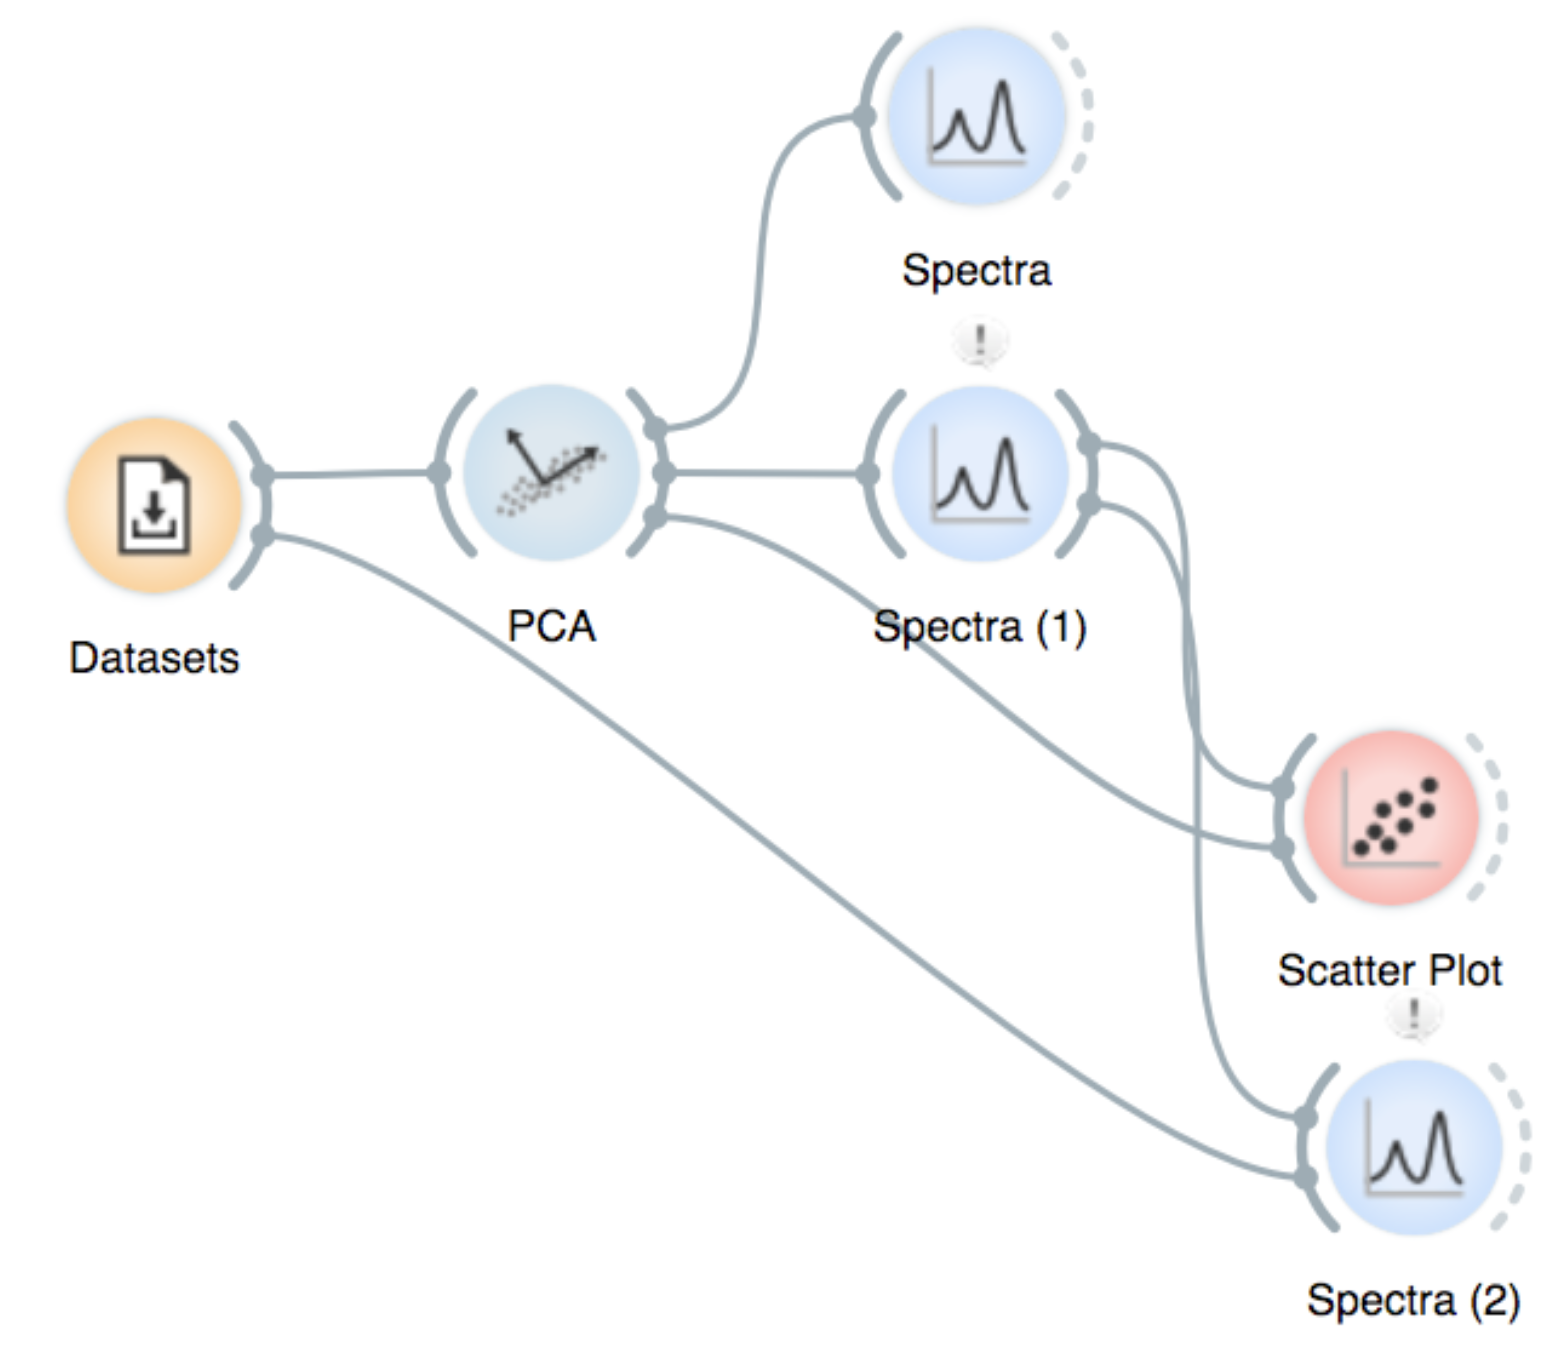
\includegraphics[width=75mm]{graphics/ch-spectral_PCA/spectral_PCA-fig4.png}%
  \label{fig:spectral-PCA-fig4}
\end{wrapfigure}

If we connect the \textit{PCA} (Transformed data output) to \textit{Spectra (1)}, we see each transformed spectrum on a line plot. As we can see, some classes have outliers. 

To find out more, select one of them: move your mouse cursor to a curve -—it will be highlighted—- and click it. The selected curve changes to a dotted line and is sent to the output. Then, connect that output to a \textit{Scatter Plot} and another \textit{Spectra} widget (both to its Data Subset inputs). We can then see the spectrum in the original space (\textit{Spectra (2)} widget) and the space of principal components (\textit{Scatter Plot}).

\begin{figure*}[h]
%   \centering
  \vspace{3cm}\stackinset{r}{0pt}{t}{+0.35\textwidth}
  {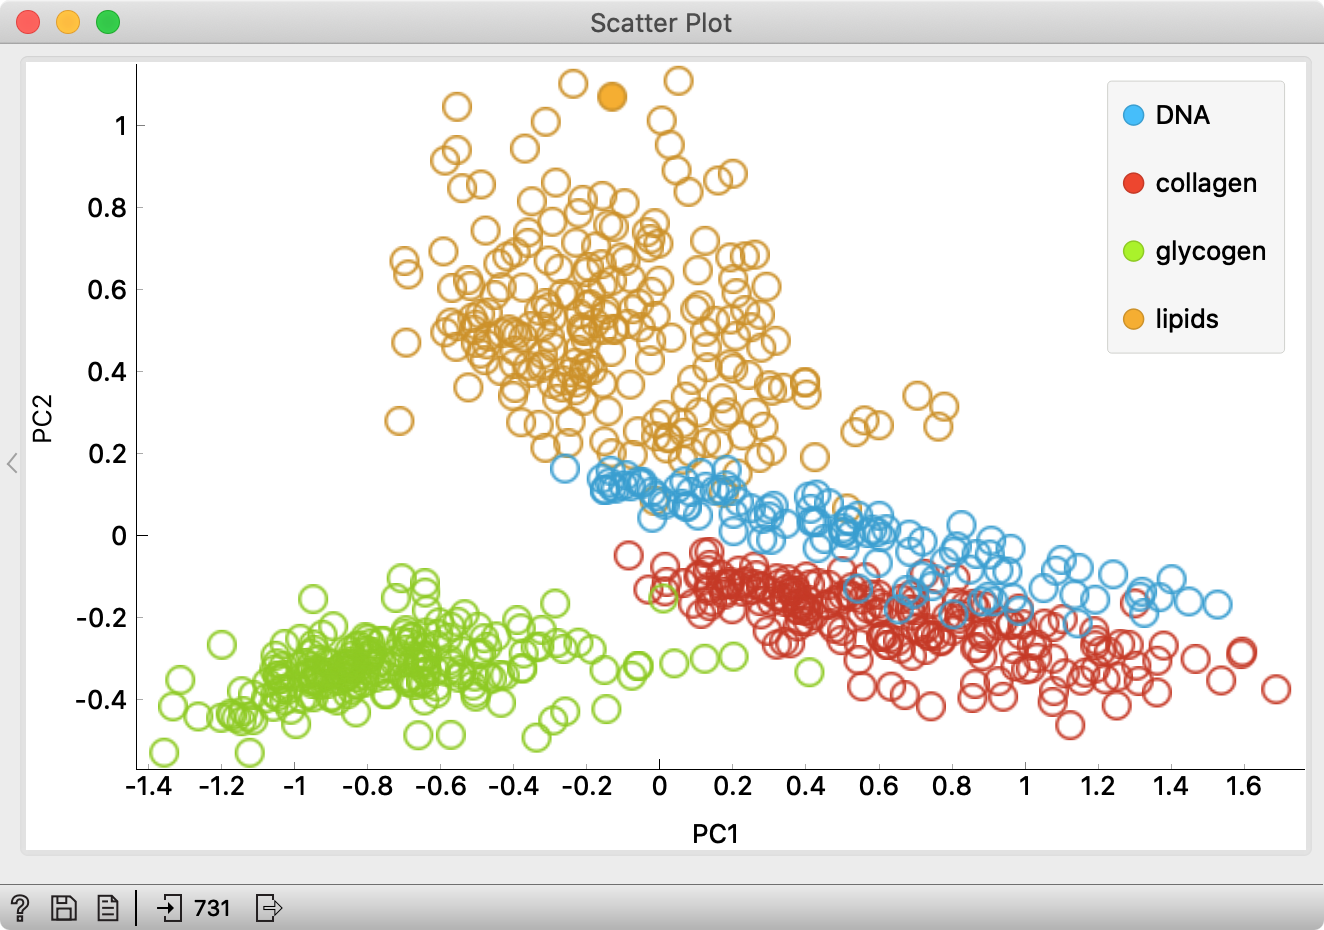
\includegraphics[width=0.48\textwidth]{graphics/ch-spectral_PCA/spectral_PCA-fig6.png}}
  {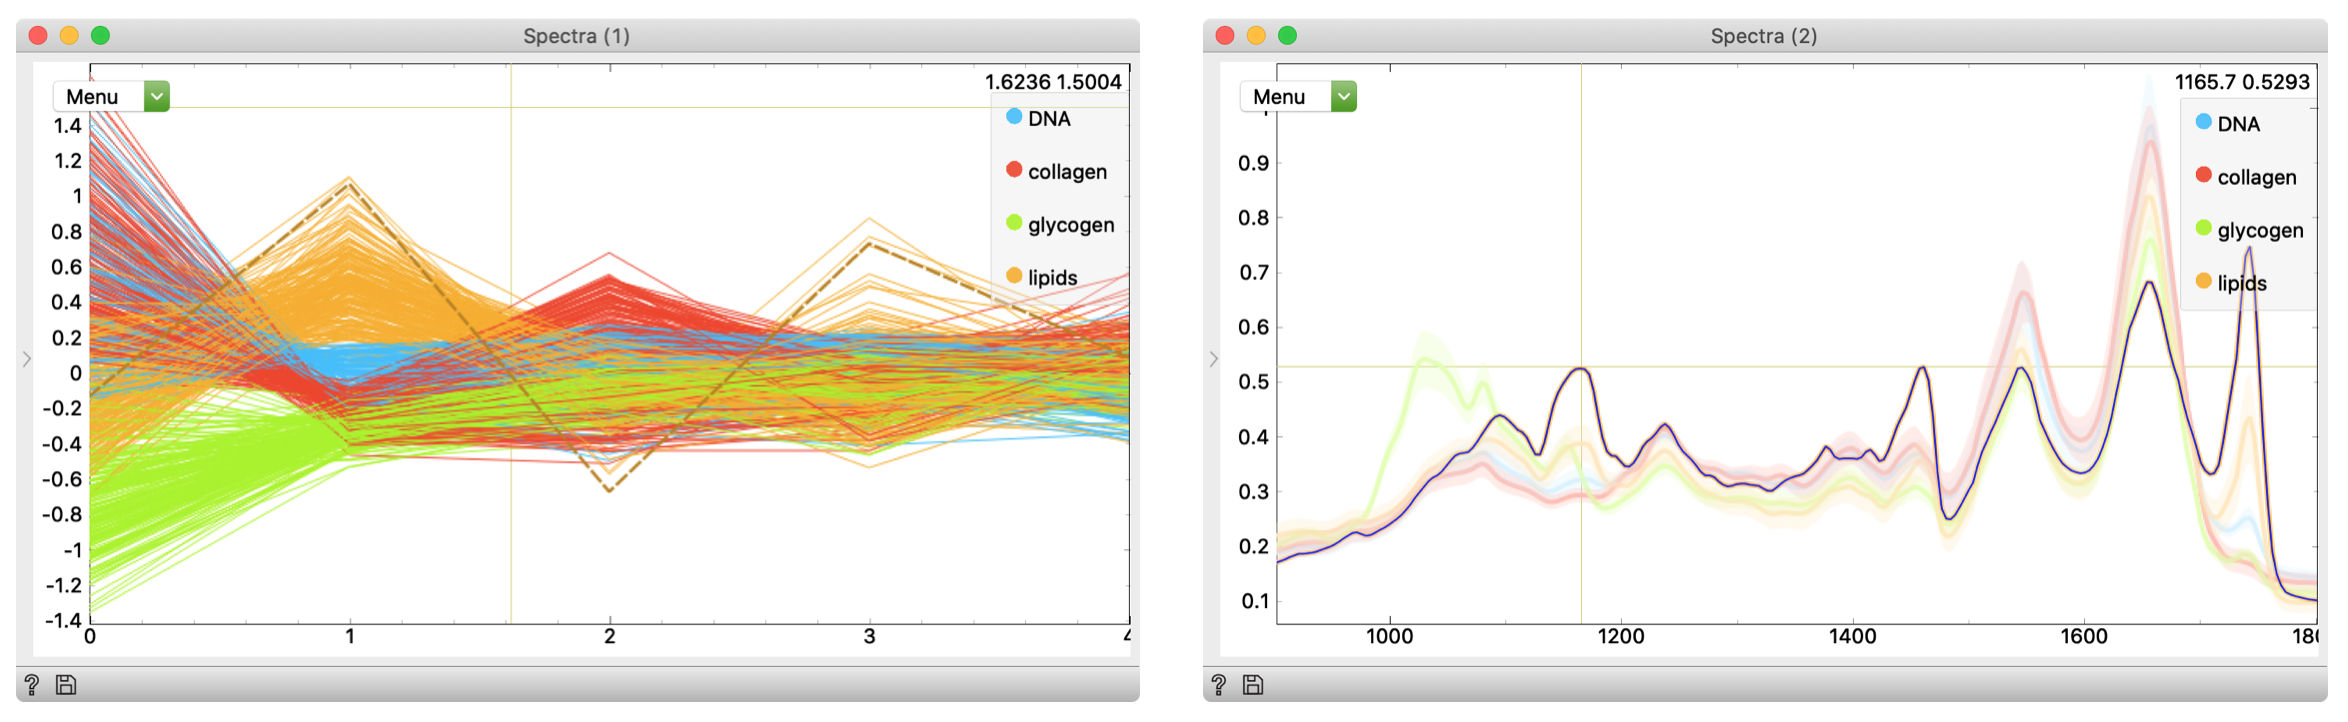
\includegraphics[width=\textwidth]{graphics/ch-spectral_PCA/spectral_PCA-fig5.png}}
  \vspace{-3.5cm}
  \caption{The selected spectrum's curve on the left is drawn with a dashed line and the corresponding original spectrum is highlighted on the right. \textit{Scatter Plot} shows the position of the selected spectrum in the PCA space.}
  \label{fig:spectral-PCA-fig5}
\end{figure*}

% Lesson 7: Hyperspectral Images
%\chapter{Working with hyperspectral data}
\label{ch:hyper_basic}


\begin{wrapfigure}{o}{0.5\textwidth}
    \centering
    \vspace{-3cm}
    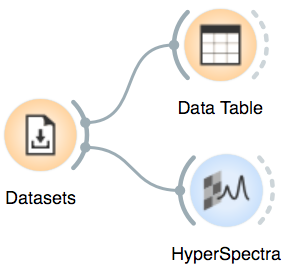
\includegraphics[width=0.45\textwidth]{graphics/ch-hyper_basic/hyperspectral-fig1.png}
    \label{fig:hyper_basic-fig1}
\end{wrapfigure}

We can also visualize hyperspectral data sets. In the \textit{Datasets} widget you will find “Liver cirrhosis” data. Connecting to a \textit{Data Table}, you will see that each spectrum contains information (in meta variables) about image positions (map\_x and map\_y). \mutation\ can recognize the image positioning features from the file automatically. Otherwise, you could set them manually in the image Menu under the \textit{Axis x} and \textit{Axis y} options. 

\begin{figure}[h]
    \centering
    % \vspace{-1cm}
    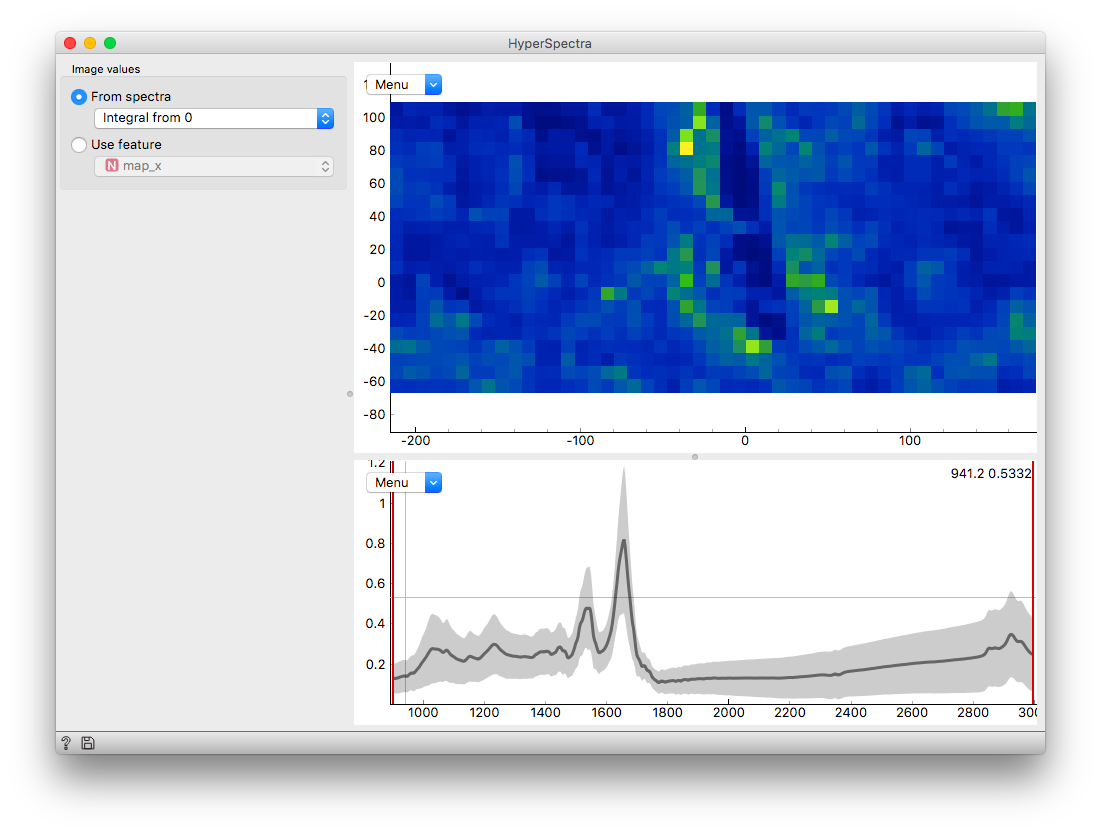
\includegraphics[width=0.8\textwidth]{graphics/ch-hyper_basic/hyperspectral-fig2.png}
    \caption{The \textit{HyperSpectra} widget has two main parts, it can show image (top) and a spectra (bottom). Explore the options on both plots in their Menus and the left panel, where you can change the visualization parameters.}
    \label{fig:hyper_basic-fig2}
\end{figure}

By default, the image is the 2D representation of the whole integral of each spectrum. To change  it, move the red lines on the spectrum plot. With the dropdown menu on the left panel you can select other representations.

\begin{figure}[h]
    \centering
    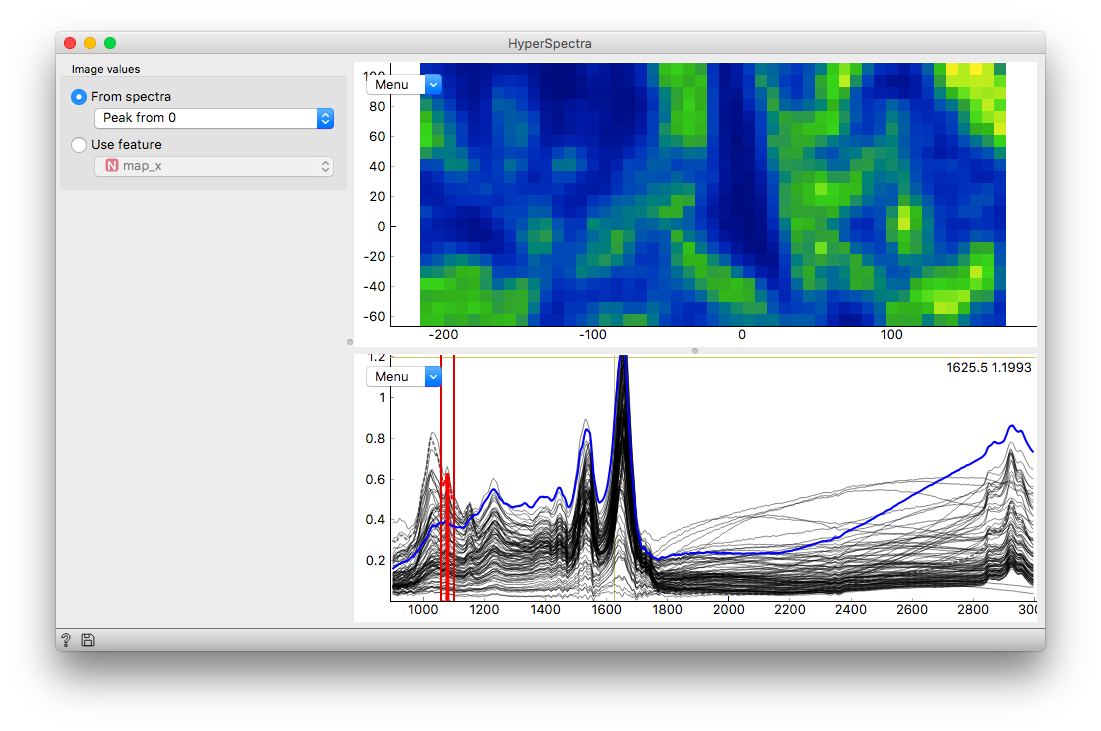
\includegraphics[width=0.8\textwidth]{graphics/ch-hyper_basic/hyperspectral-fig3.png}
    \caption{To view the plotted integrals, set the spectra display to show individual spectra and click a spectrum. Integrals for the selected spectrum are shaded.}
    \label{fig:hyper_basic-fig3}
\end{figure}

% Lesson 8: Spectral Preprocessing
%\chapter{Preprocessing spectal data}
\label{ch:spectral_preprocessing}


\begin{wrapfigure}{o}{0.63\textwidth}
    \centering
    \vspace{-3.4cm}
    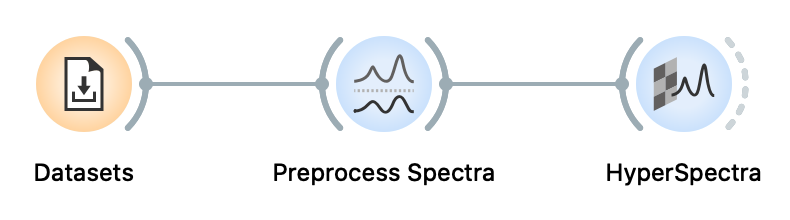
\includegraphics[width=0.75\textwidth]{graphics/ch-spectral_preprocessing/spectral_preprocessing-fig1.png}
    \label{fig:spectral_preprocessing-fig1}
\end{wrapfigure}

Preprocessing spectra is a very important step of data analysis. \mutation\ has a widget, \textit{Preprocessing}, dedicated to different methods.The spectra from the “Liver cirrhosis” data set could use some preprocessing. There is some scattering visible and perhaps there are some artifacts due to sample thickness varying slightly.

\begin{figure}[h]
    \centering
    % \vspace{-1cm}
    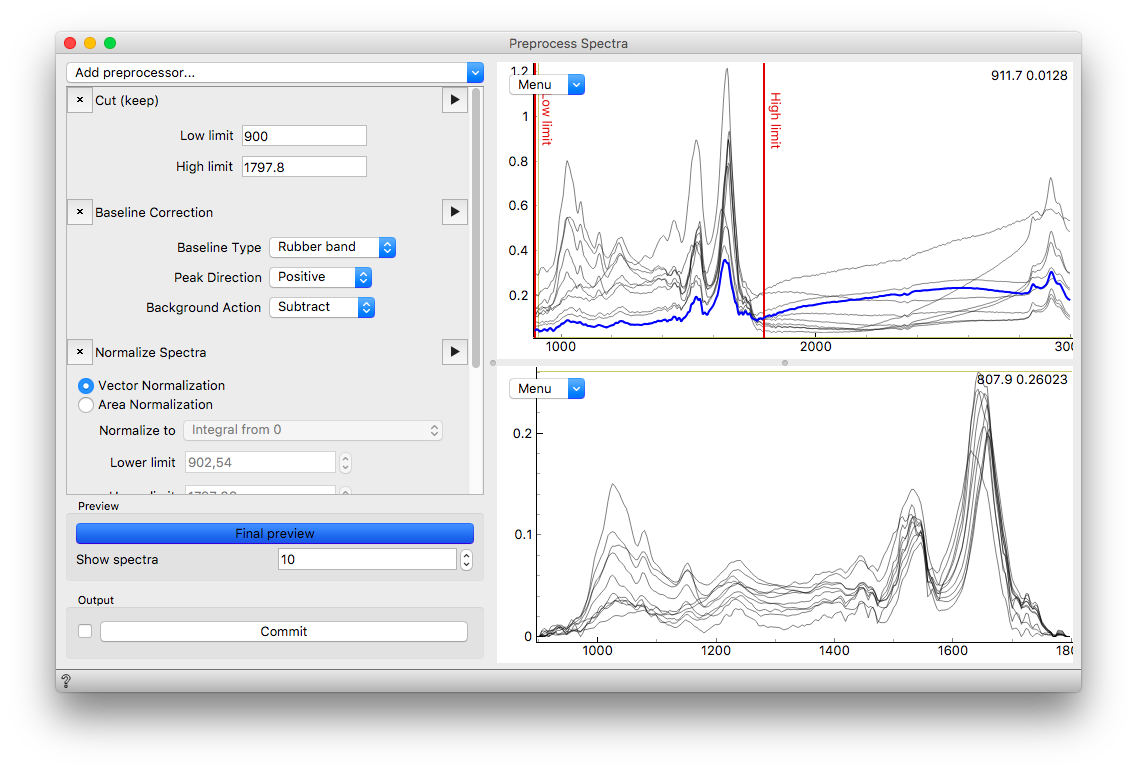
\includegraphics[width=\textwidth]{graphics/ch-spectral_preprocessing/spectral_preprocessing-fig2.png}
    \caption{You can add preprocessing steps from the top dropdown menu of the left panel. Then, it is possible to drag them up and down to change their order. Each preprocessor has its own parameters. In the example here we show how the Baseline correction is done: you can simply change the baseline points by dragging the red lines in the top spectrum panel. Each stage can be previewed by clicking the small triangle.}
    \label{fig:spectral_preprocessing-fig2}
\end{figure}

Let's see the result of our preprocessing in a \textit{HyperSpectra} widget.

\begin{figure}[h]
    \centering
    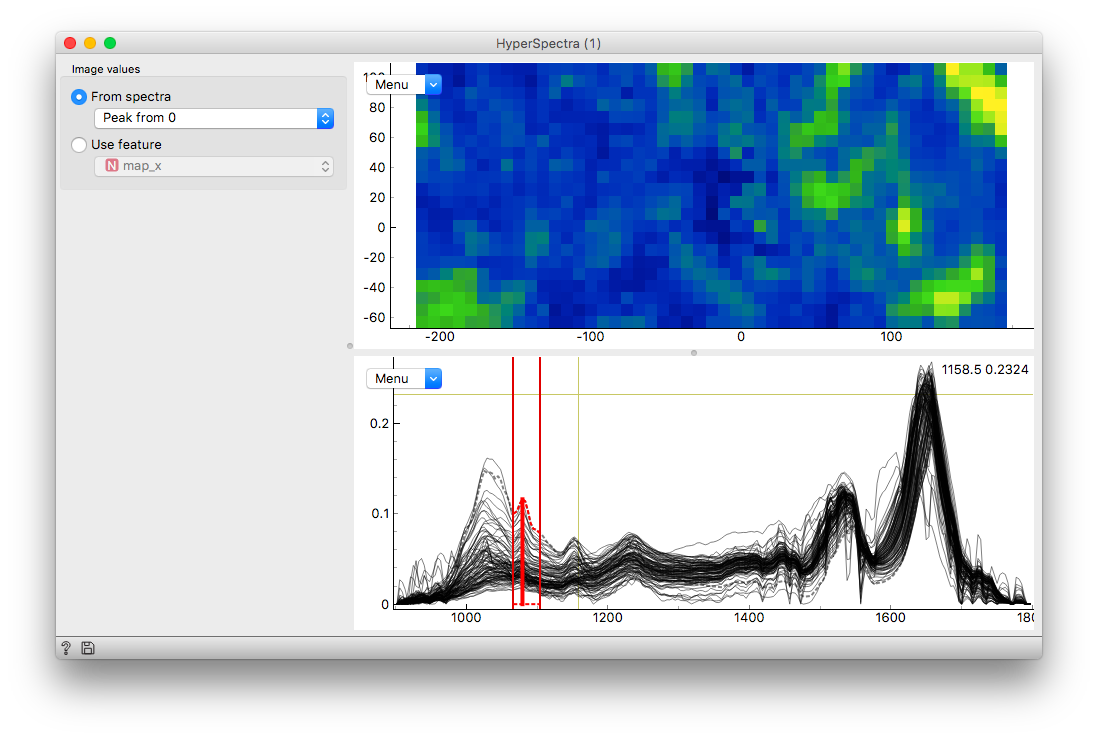
\includegraphics[width=0.9\textwidth]{graphics/ch-spectral_preprocessing/spectral_preprocessing-fig3.png}
    \caption{The preprocessed data in \textit{HyperSpectra}. Did we gain anything? To investigate why the blue island disappeared, click on a pixel in it to see its spectrum.}
    \label{fig:spectral_preprocessing-fig3}
\end{figure}

% Lesson 9: Integrals and Ratios
%\chapter{Integrals and ratios}
\label{ch:spectral_preprocessing}


\begin{wrapfigure}{o}{0.72\textwidth}
    \centering
    \vspace{-3cm}
    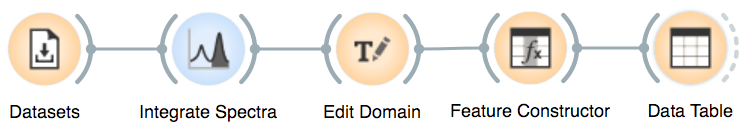
\includegraphics[width=0.85\textwidth]{graphics/ch-integrals-ratios/integrals-ratios-fig1.png}
    \label{fig:integrals-ratios-fig1}
\end{wrapfigure}

Peak integration is an essential element of spectroscopy for measuring concentrations, spectral contributions, etc. 

\begin{wrapfigure}{o}{0.95\textwidth}
    \centering
    % \vspace{-1cm}
    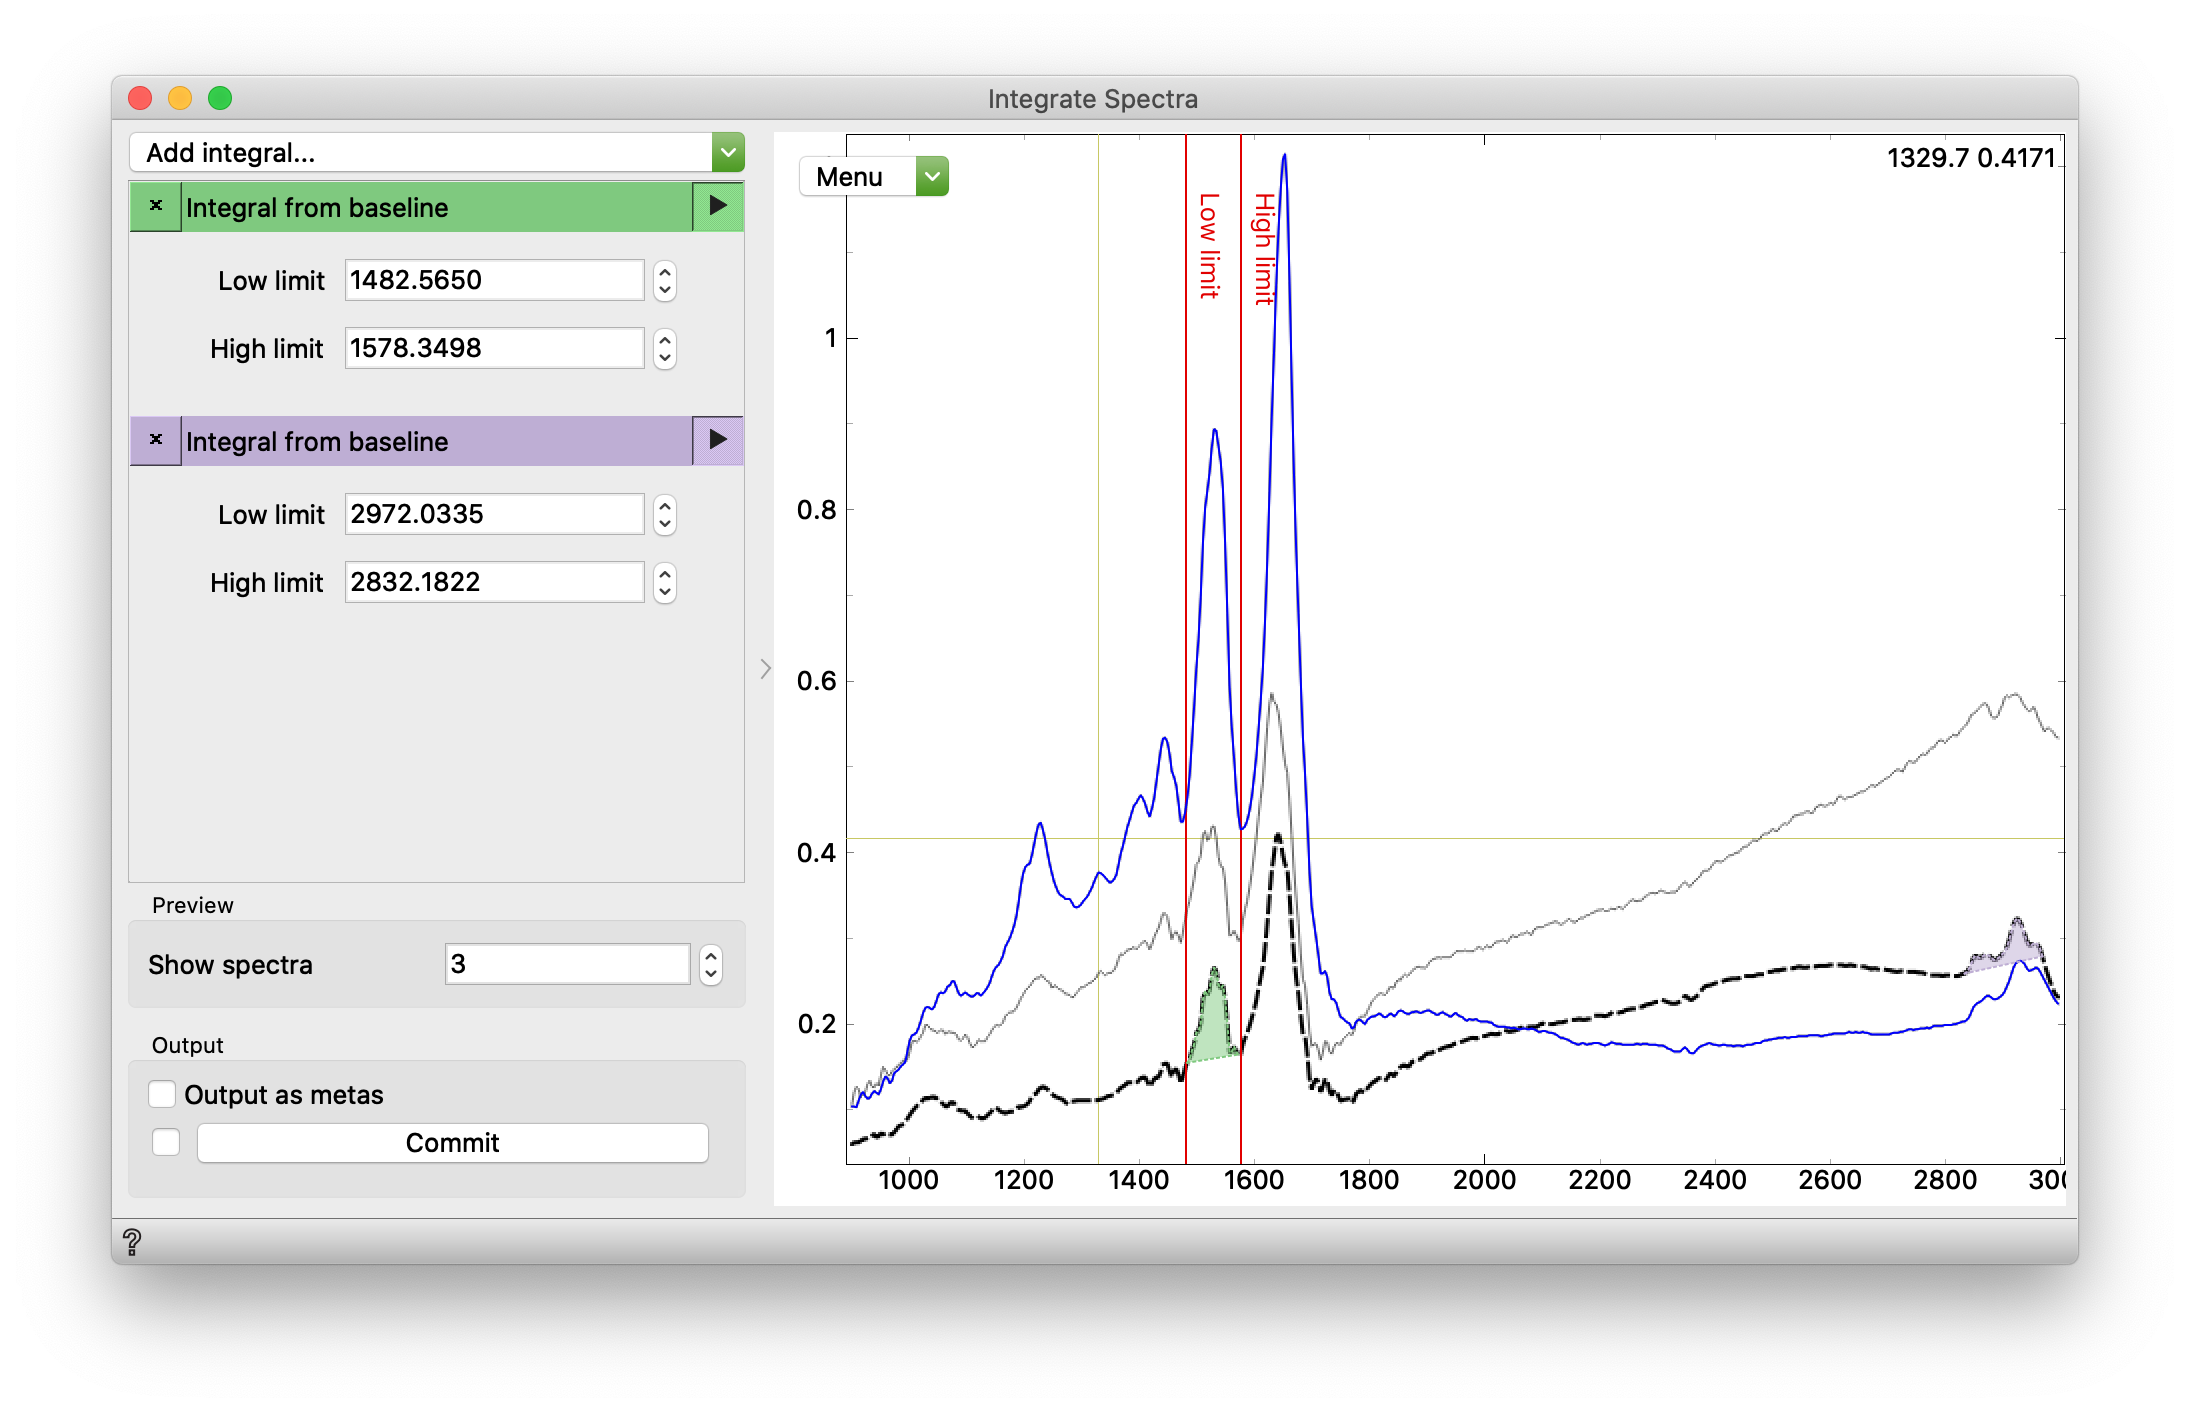
\includegraphics[width=\textwidth]{graphics/ch-integrals-ratios/integrals-ratios-fig2.png}
    \caption{To display a preview, select a spectrum and enable preview of individual integrals with their play buttons.}
    \label{fig:integrals-ratios-fig2}
\end{wrapfigure}

To compute integrals, we use the \textit{Integrate Spectra} widget. Let’s compute the ratios of two integrals to establish an internal standard in our dataset. Add two integrals and then feed them into the \textit{Feature Constructor} (\textit{Edit Domain} is optional—we use it to simplify column names). In \textit{Feature Constructor}, we can create new numeric features with Python expressions.
To work with Feature Constructor more easily, uncheck “Output as metas”, which will replace the original spectra with their integrals (and reduce the number of columns in your data).
We can use \textit{Feature Constructor} whenever we would like to create a new column from existing data. 

\begin{figure}[h]
\vspace{-0.5cm}

\stackinset{r}{-0.65\linewidth}{t}{+0.15\linewidth}
% {r} is left-right
% {t} is top-bottom
  {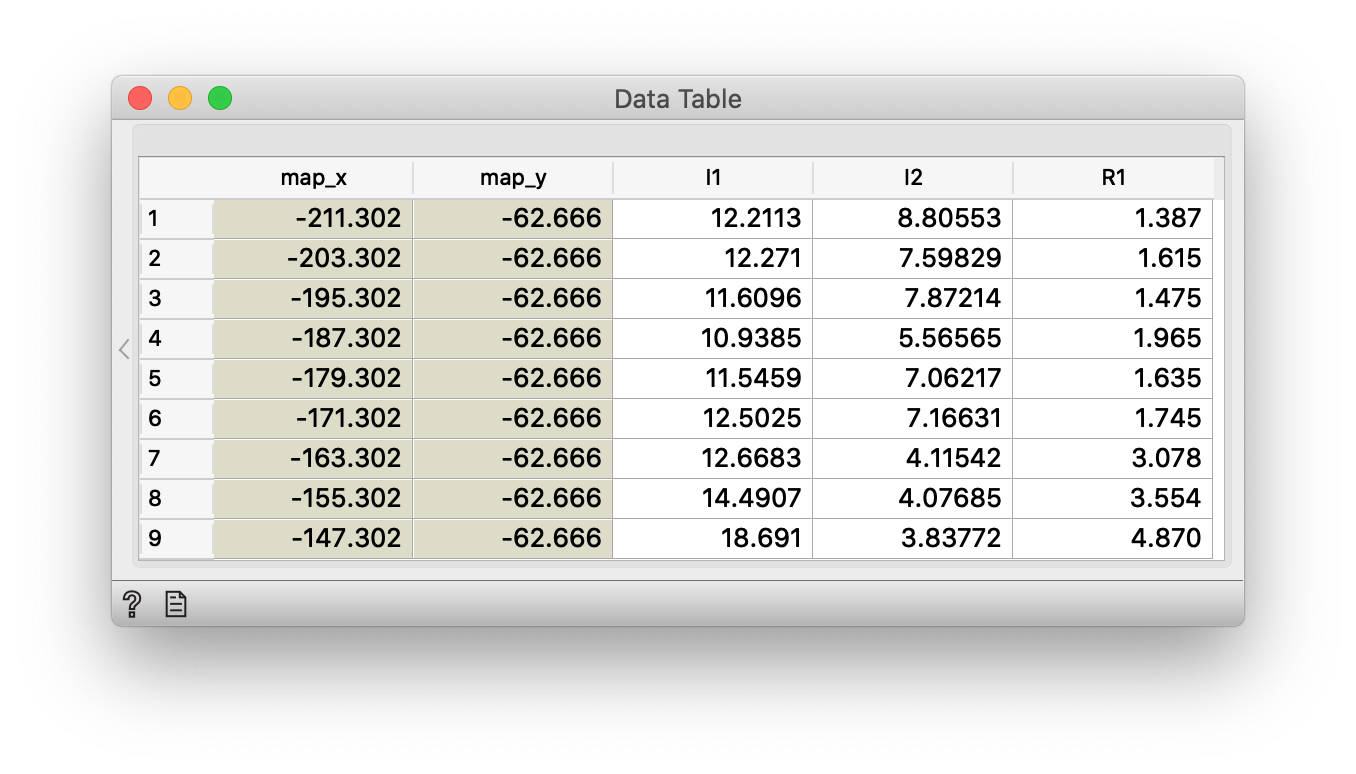
\includegraphics[scale=0.45]{graphics/ch-integrals-ratios/integrals-ratios-fig4.png}}
  {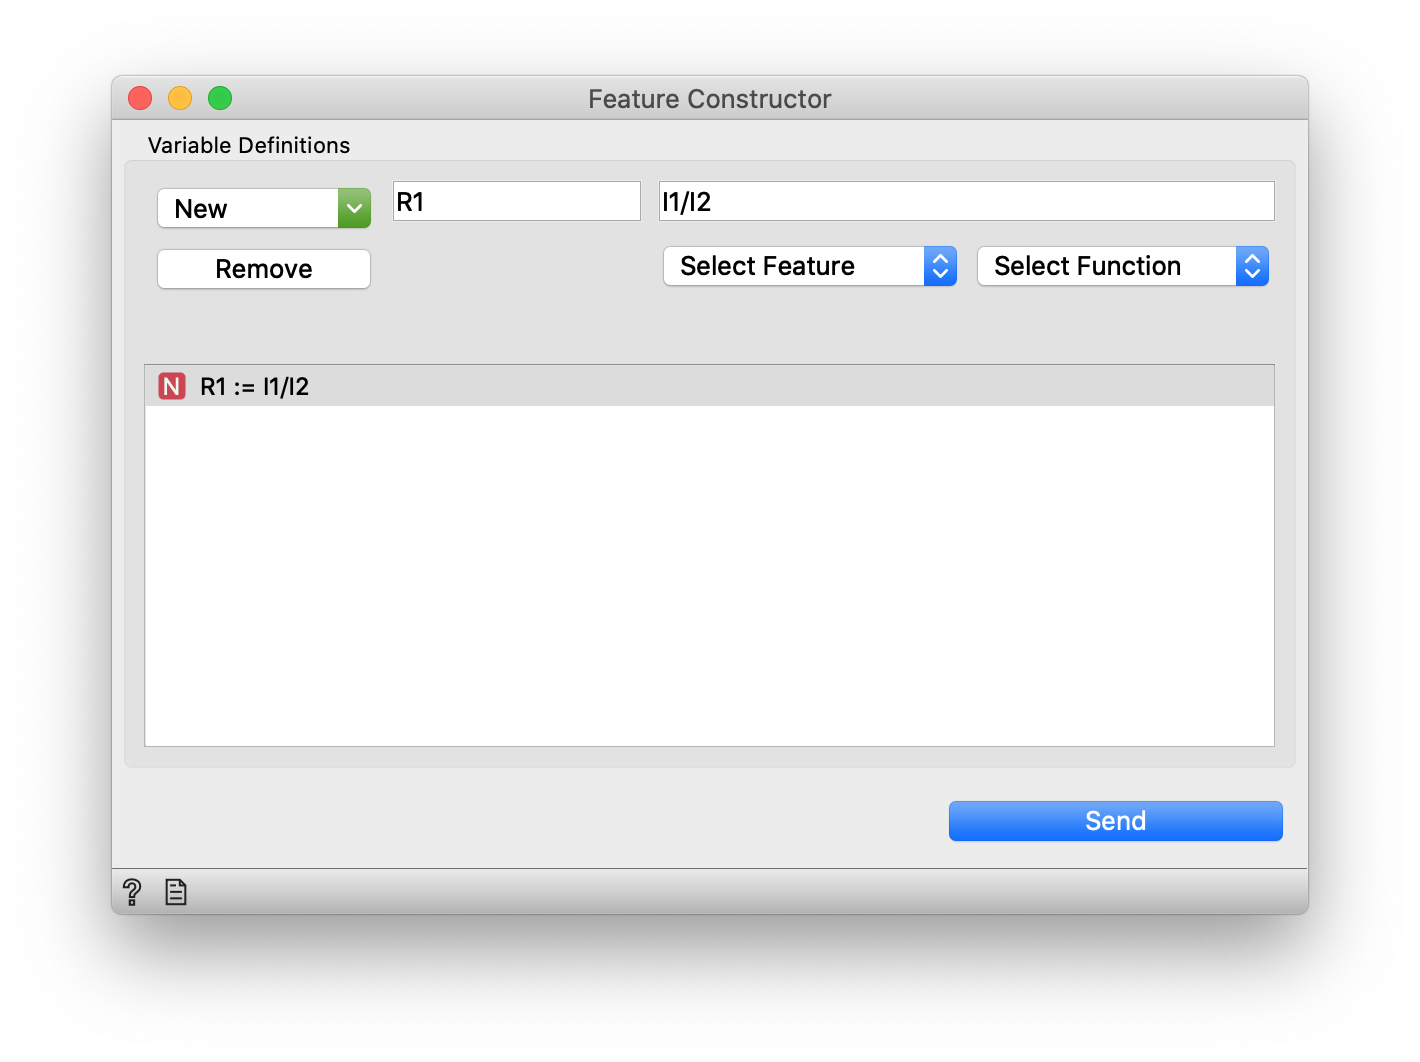
\includegraphics[scale=0.4]{graphics/ch-integrals-ratios/integrals-ratios-fig3.png}}
  \caption{We added a Numeric feature, the ratio of I1 and I2 called R1.}
  \label{fig:spectral-PCA-fig2}
\end{figure}

\noindent The produced data can be inspected by connecting other widgets.
% Lesson 10: Classification
%\chapter{Classification}
\label{ch:classification}

We have seen the iris data before. \marginnote{We call the variable we wish to predict a target variable, or an outcome or, in traditional machine learning terminology, a class. Hence we talk about classification, classifiers, classification trees...} We wanted to predict varieties based on measurements---but we actually did not make any predictions. We observed some potentially interesting relations between the features and the varieties, but have never constructed an actual model.

Let us create one now.

\begin{figure}[h]
    \centering
    \vspace{-0.2cm}
    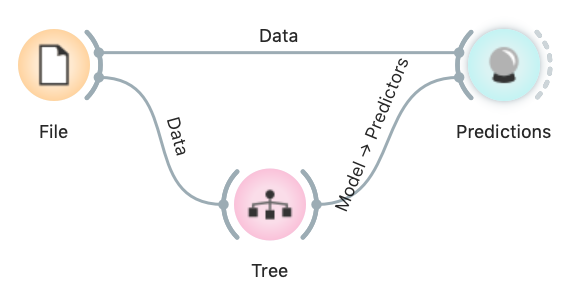
\includegraphics[scale=0.4]{graphics/ch-classification/predictions-workflow.png}
    \caption{Something in this workflow is conceptually wrong. Can you guess what?}
    \label{fig:spectral_preprocessing-fig2}
\end{figure}

\begin{wrapfigure}{o}{1.1\textwidth}
    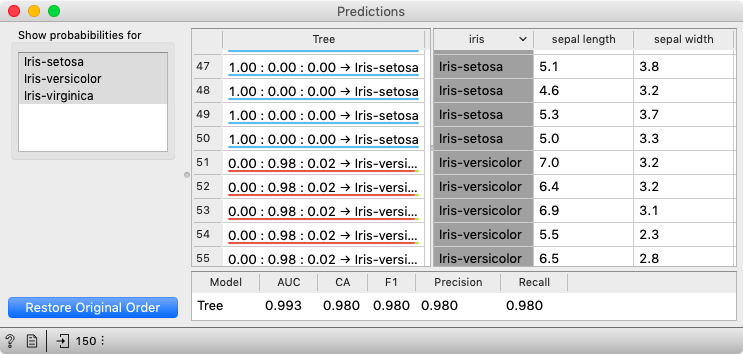
\includegraphics[scale=0.4]{graphics/ch-classification/predictions.png}
    \label{fig:classification-predictions}
\end{wrapfigure}

The data is fed into the Tree widget, which infers a classification model and gives it to the Predictions widget. Note that unlike in our past workflows, in which the communication between widgets included only the data, we here have a channel that carries a predictive model.

The Predictions widget also receives the data from the File widget. The widget uses the model to make predictions about the data and shows them in the table.

How correct are these predictions? Do we have a good model? How can we tell?

But (and even before answering these very important questions), what is a classification tree? And how does Orange create one? Is this algorithm something we should really use?

So many questions to answer!

% Lesson 11: Classification Trees
%\chapter{Classification Trees}
\label{ch:classification-trees}

In the previous lesson, we used a classification tree,
\marginnote{Classification trees were hugely popular in the early years of machine learning, when they were first independently proposed by the engineer Ross Quinlan (C4.5) and a group of statisticians (CART), including the father of random forests Leo Brieman.}
one of the oldest, but still popular, machine learning methods. We like it since the method is easy to explain and gives rise to random forests, one of the most accurate machine learning techniques (more on this later). So, what kind of model is a classification tree?

Let us load \textit{iris} data set, build a tree (widget \widget{Tree}) and visualize it in a \widget{Tree Viewer}.

\begin{figure}[h]
    \centering
    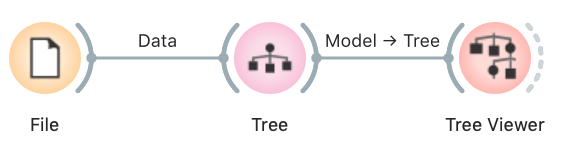
\includegraphics[scale=0.4]{graphics/ch-classification_trees/workflow-tree-viewer.png}
\end{figure}

\begin{figure*}[h]
    \vspace{-0.4cm}
    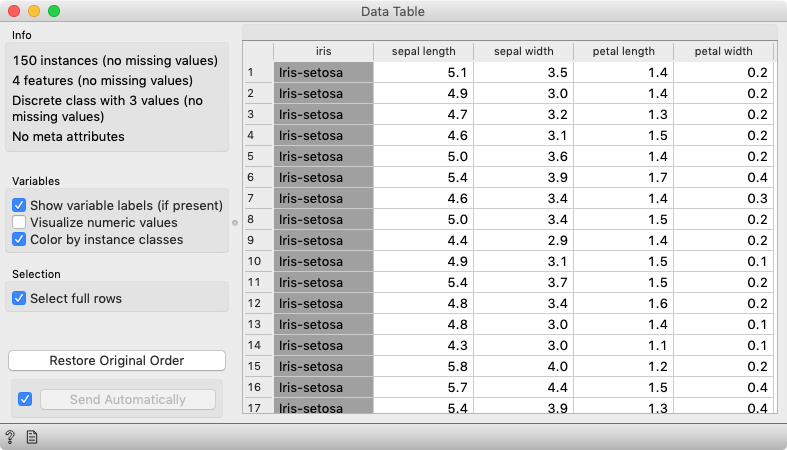
\includegraphics[scale=0.35]{graphics/ch-classification_trees/iris-data.png}
    \label{fig:classification-predictions}
\end{figure*}

\begin{wrapfigure}{o}{1.1\textwidth}
    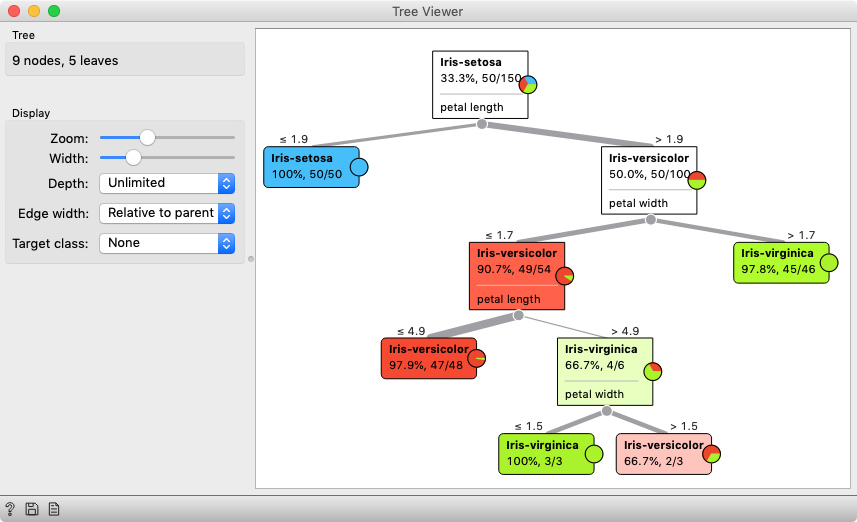
\includegraphics[scale=0.35]{graphics/ch-classification_trees/tree-viewer.png}
    \label{fig:classification-predictions}
\end{wrapfigure}

We read the tree from top to bottom. Looks like the column \textit{petal length} best separates iris variety \textit{setosa} from the others, while \textit{petal width} then almost perfectly separates the remaining two varieties.

Trees place the most useful feature at the root. What would be the most useful feature? The feature that splits the data into two purest possible subsets. It then splits both subsets further, again by their most useful features, and keeps doing so until it reaches subsets in which all data belongs to the same class (leaf nodes in strong blue or red) or until it runs out of data instances to split or out of useful features (the two leaf nodes in white).

We still have not been very explicit about what we mean by ``the most useful'' feature. There are many ways to measure the quality of features, based on how well they distinguish between classes. We will illustrate the general idea with information gain. We can compute this measure in Orange using the \widget{Rank} widget \marginnote{The \widget{Rank} widget can be used on its own to show the best predicting features. Say, to figure out which genes are best predictors of the phenotype in some gene expression data set.}, which estimates the quality of data features and ranks them according to how informative they are about the class. We can either estimate the information gain from the whole data set, or compute it on data corresponding to an internal node of the classification tree in the \widget{Tree Viewer}. In the following example we use the \textit{Sailing} data set.

\begin{figure}[h]
    \centering
    \includegraphics[scale=0.4]{graphics/ch-classification_trees/workflow-rank.png}
    \caption{The \widget{Datasets} widget is set to load the \textit{Sailing} data set. To use the second \widget{Rank}, select a node in the \widget{Tree Viewer}.}
\end{figure}

Besides the information gain, \widget{Rank} displays several other measures (including Gain Ratio and Gini), which are often quite in agreement and were invented to better handle discrete features with many different values.

\begin{figure}[h]
    \centering
    \vspace{-0.2cm}
    \includegraphics[scale=0.4]{graphics/ch-classification_trees/rank.png}
    \caption{For the whole \textit{Sailing} data set, \textit{Company} is the most class-informative feature according to all measures shown.}
\end{figure}

% Lesson 12: Model Inspection - merged to classification trees
% Lesson 13: Naive Bayes
% \chapter{Naive Bayes}
\label{ch:naive_bayes}

Naive Bayes \marginnote{Naive Bayes assumes class-wise independent features. For a data set where features would actually be independent, which rarely happens in practice, the naive Bayes would be the ideal classifier.} is also a classification method. To see how naive Bayes works, we will use a data set on passengers’ survival in the Titanic disaster of 1912. The \textit{Titanic} data set describes 2201 passengers, with their tickets (first, second, thirds class or crew), age and gender.

\begin{figure}[h]
    \centering
    \vspace{-0.2cm}
    \includegraphics[scale=0.4]{graphics/ch-naive_bayes/workflow.png}
\end{figure}

We inspect naive Bayes models with the \widget{Nomogram} widget. There, we se a scale ‘Points’ and scales for each feature. Below we can see probabilities. Note the ‘Target class’ in upper left corner. If it is set to ‘yes’, the widget will show the probability that a passenger survived.

The nomogram shows that gender was the most important feature for survival. If we move the blue dot to ‘female’, the survival probability increases to 73\%. Furthermore, if that woman also travelled in the first class, she survived with probability of 90\%. The bottom scales show the conversion from feature contributions to probability.

\begin{figure}[h]
    \centering
    \includegraphics[scale=0.45]{graphics/ch-naive_bayes/nomogram.png}
    \caption{According to the probability theory individual contributions should be multiplied. Nomograms get around this by working in a log-space: a sum in the log-space is equivalent to multiplication in the original space. Therefore nomograms sum contributions (in the log-space) of all feature values and then convert them back to probability.}
\end{figure}

% Lesson 14: Classification Accuracy
\chapter{Classification Accuracy}
\label{ch:classification_accuracy}

Now that we know what classification trees are, the next question is what is the quality of their predictions. For beginning, we need to define what we mean by quality. In classification, the simplest measure of quality is classification \marginnote{$\mathrm{accuracy}=\frac{\# \{\mathrm{correct}\}}{\# \{\mathrm{all}\}}$} accuracy expressed as the proportion of data instances for which the classifier correctly guessed the value of the class. Let's see if we can estimate, or at least get a feeling for, classification accuracy with the widgets we already know.

\begin{wrapfigure}{o}{0.85\textwidth}
    \vspace{-0.5cm}
    \includegraphics[scale=0.4]{graphics/ch-classification_accuracy/workflow.png}
\end{wrapfigure}

Let us try this schema with the \textit{iris} data set. The \widget{Predictions} widget outputs a data table augmented with a column that includes predictions. In the \widget{Data Table} widget, we can sort the data by any of these two columns, and manually select data instances where the values of these two features are different (this would not work on big data). Roughly, visually estimating the accuracy of predictions is straightforward in the \widget{Distribution} widget, if we set the features in view appropriately.

For precise statistics of correctly and incorrectly classified examples open the \widget{Confusion Matrix} widget.

\begin{figure*}[h]
    \centering
    \newcommand{\predictions}{\includegraphics[scale=0.40]{graphics/ch-classification_accuracy/predictions2.png}}
    \newcommand{\distributions}{\includegraphics[scale=0.25]{graphics/ch-classification_accuracy/distributions.png}}
    \newcommand{\confusion}{\includegraphics[scale=0.25]{graphics/ch-classification_accuracy/confusion.png}}
    \infinitewidthbox{
    \stackinset{r}{-0.35\linewidth}{b}{-0.05\linewidth}{\confusion}
    {\stackinset{r}{-0.35\linewidth}{b}{+0.15\linewidth}{\distributions}{\predictions}}\hspace{7cm}
    }
    \caption{The \widget{Confusion Matrix} shows 3 incorrectly classified examples, which makes the accuracy $(150-3)/150 = 98\%$.}
\end{figure*}

%Lesson 15: How to Cheat
\chapter{How to Cheat}
\label{ch:how_to_cheat}

\begin{wrapfigure}{o}{0.85\textwidth}
    \includegraphics[scale=0.4]{graphics/ch-how_to_cheat/workflow-randomize.png}
\end{wrapfigure}

At this stage, \marginnote[-2cm]{This lesson has a strange title and it is not obvious why it was chosen. Maybe you, the reader, should tell us what does this lesson have to do with cheating.} the classification tree looks very good. There’s only one data point where it makes a mistake. Can we mess up the data set so bad that the trees will ultimately fail? Like, remove any existing correlation between features and the class? We can! There’s the \widget{Randomize} widget with class shuffling. Check out the chaos it creates in the \widget{Scatter Plot} visualization where there were nice clusters before randomization!

\begin{figure*}[h]
    \infinitewidthbox{
    \includegraphics[scale=0.3]{graphics/ch-how_to_cheat/scatterplot_iris.png}
    \includegraphics[scale=0.4]{graphics/ch-how_to_cheat/randomize100.png}
    \includegraphics[scale=0.3]{graphics/ch-how_to_cheat/scatterplot_iris_random.png}
    }
    \caption{Left: scatter plot of the \textit{Iris} data set before randomization; right: scatter plot after shuffling 100\% of rows.}
\end{figure*}

Fine. There can be no classifier that can model this mess, right? Let’s make sure.

\begin{figure}[h]
    \includegraphics[scale=0.4]{graphics/ch-how_to_cheat/workflow_classification.png}
\end{figure}

\begin{wrapfigure}{o}{0.85\textwidth}
    \includegraphics[scale=0.35]{graphics/ch-how_to_cheat/confusion_randomized.png}
\end{wrapfigure}

And the result? Here is a screenshot of the \widget{Confusion Matrix}.

Most unusual. Despite shuffling all the classes, which destroyed any connection between features and the class variable, about 80\% of predictions were still correct.

\clearpage

Can we further improve accuracy on the shuffled data? Let us try to change some properties of the induced trees: in the \widget{Tree} widget, disable all early stopping criteria.

\begin{figure}[h]
    \includegraphics[scale=0.35]{graphics/ch-how_to_cheat/better_tree.png}
    \includegraphics[scale=0.35]{graphics/ch-how_to_cheat/confusion_randomized_better.png}
    \caption{After we disable 2--4 check box in the \widget{Tree} widget, our classifier starts behaving almost perfectly.}
\end{figure}


Wow, almost no mistakes now. How is this possible? On a class-randomized data set?

\begin{wrapfigure}{o}{0.85\textwidth}
    \includegraphics[scale=0.35]{graphics/ch-how_to_cheat/tree_viewer.png}
    \caption{In the build tree, there are 75 leaves. Remember, there are only 150 rows in the \textit{Iris} data set.}
\end{wrapfigure}

To find the answer to this riddle, open the \widget{Tree Viewer} and check out the tree. How many nodes does it have? Are there many data instances in the leaf nodes?

Looks like the tree just memorized every data instance from the data set. No wonder the predictions were right. The tree makes no sense, and it is complex because it simply remembered everything.

Ha, if this is so, if a classifier remembers everything from a data set but without discovering any general patterns, it should perform miserably on any new data set. Let us check this out. We will split our data set into two sets, training and testing, train the classification tree on the training data set and then estimate its accuracy on the test data set.

\begin{figure}[h]
    \includegraphics[scale=0.35]{graphics/ch-how_to_cheat/workflow_data_sampler.png}
    \caption{Connect the \widget{Data Sampler} widget carefully. The \widget{Data Sampler} splits the data to a sample and out-of-sample (so called remaining data). The sample was given to the \widget{Tree} widget, while the remaining data was handed to the \widget{Predictions} widget. Set the \widget{Data Sampler} so that the size of these two data sets is about equal.}
\end{figure}

Let’s check how the \widget{Confusion Matrix} looks after testing the classifier on the test data.

\begin{figure}[h]
    \includegraphics[scale=0.35]{graphics/ch-how_to_cheat/confusion_sampler.png}
    \caption{Confusion matrix if we estimate accuracy on a data set that was not used in learning.}
\end{figure}

The first two classes are a complete fail. The predictions for ribosomal genes are a bit better, but still with lots of mistakes. On the class-randomized training data our classifier fails miserably. Finally, just as we would expect.

We have just learned that we need to train the classifiers on the training set and then test it on a separate test set to really measure performance of a classification technique. With this test, we can distinguish between those classifiers that just memorize the training data and those that actually learn a general model.

Learning is not only memorizing. Rather, it is discovering patterns that govern the data and apply to new data as well. To estimate the accuracy of a classifier, we therefore need a separate test set. This estimate should not depend on just one division of the input data set to training and test set (here’s a place for cheating as well). Instead, we need to repeat the process of estimation several times, each time on a different train/test set and report on the average score.
%Marko % Lesson 16: Random Forests
%Marko % Lesson 17: Cross-Validation
%Marko% Lesson 18: Hierarchical Clustering
%Marko % Lesson 19: Animal Kingdom
% Lesson 20: Classification of Spectra
  %%% 2020.04.19 Problem with workflow #2 in this chapter! Orange 3.26.0.dev
%\chapter{Classification of Spectra}
\label{ch:spectra_classification}

\begin{wrapfigure}{o}{0.82\textwidth}
    \centering
    \vspace{-3.4cm}
    \includegraphics[width=0.95\textwidth]{graphics/ch-spectra_classification/sp_classification-fig1.png}
    \label{fig:spectra_classification-fig1}
\end{wrapfigure}


Let’s open the collagen data set again and see how well can logistic regression predict its four classes. Straightforward, right? Connect \widget{Datasets}, \widget{Logistic Regression}, \widget{Predictions}, \widget{Confusion Matrix} and that's it. We would also like to do some spectral processing (we will only keep the columns for wavenumbers between 1500\wn and 1800\wn).

\begin{figure}[h]
\hspace{-1cm}\stackinset{r}{-0.7\linewidth}{t}{+0.25\linewidth}
  {\includegraphics[scale=0.35]{graphics/ch-spectra_classification/sp_classification-fig2b.png}}
  {\includegraphics[scale=0.45]{graphics/ch-spectra_classification/sp_classification-fig2a_.png}}
  \caption{The \widget{Spectra} widget shows wrong predictions for the DNA class.}
  \label{fig:spectra_classification-fig2}
\end{figure}

Let’s not forget that it is pointless to predict for the same data as we used for learning. We could either  use a \widget{Data Sampler} and connect its Sample output to \widget{Preprocess Spectra} and Remaining output to \widget{Predictions}, or obtain predictions from the \widget{Test and Score} widget.
\widget{Confusion Matrix} now shows the mistakes of the model (scored with cross-validation). We can select them and inspect them further in a \widget{Spectra} widget. Here we colored them by the predicted class (see the Menu). 

\begin{wrapfigure}{o}{1.1\textwidth}
  \centering
  \includegraphics[width=1.1\textwidth]{graphics/ch-spectra_classification/sp_classification-fig3.png}%
  \label{fig:spectra_classification-fig3}
\end{wrapfigure}
But how does the model make its decisions? We already inspected a different model, classification tree, where each node represents a decision on a value of a column.  \widget{Logistic regression} works differently. On the training data it computes weights for all columns (wavelengths), which are then used for prediction, where values are multiplied with weights. To see the weights, connect \widget{Logistic Regression} to a \widget{Data Table}. 

\begin{wrapfigure}{o}{0.9\textwidth}
%  \centering
  \vspace{-0.7cm}
  \includegraphics[width=0.9\textwidth]{graphics/ch-spectra_classification/sp_classification-fig4.png}
  \label{fig:spectra_classification-fig4}
\end{wrapfigure}
We get a table that is hard to understand. What if we visualize it? First, \widget{Transpose} the data. Then, use \widget{Select Columns} to make the visualization prettier: in the widget remove the intercept.

Now, open \widget{Logistic Regression} and try changing its parameters. Observe the effect on the weights.

\begin{figure}[h]
\hspace{-1cm}\stackinset{r}{0\linewidth}{t}{-0.22\linewidth}
  {\includegraphics[scale=0.35]{graphics/ch-spectra_classification/sp_classification-fig5a.png}}
  {\includegraphics[scale=0.35]{graphics/ch-spectra_classification/sp_classification-fig5b.png}}
  \label{fig:spectra_classification-fig5}
\end{figure}

%Marko % Lesson 21: New and Different Test Data
% Lesson 22: Clustering Spectral Images
%\chapter{Clustering Spectral Images}
\label{ch:spectra_image_clustering}

\begin{wrapfigure}{o}{0.63\textwidth}
    \centering
    \vspace{-3.3cm}
    \includegraphics[width=0.75\textwidth]{graphics/ch-spectra_image_clustering/sp_image_clustering-fig1.png}
    \label{fig:spectra_image_clustering-fig1}
\end{wrapfigure}

We have already seen hierarchical clustering. Another clustering algorithm, k-Means, is much faster for data with lots of rows, like images, which contain a row (a spectrum) for each pixel. Still, for the liver-cirrhosis data, both approaches are fast. Here, we use \widget{k-Means} with k=3 clusters. 

\begin{figure}[h]
\vspace{-0.5cm}
\hspace{-1cm}\stackinset{r}{-1.15\linewidth}{t}{0.025\linewidth}
  {\includegraphics[scale=0.33]{graphics/ch-spectra_image_clustering/sp_image_clustering-fig2b.png}}
  {\includegraphics[scale=0.55]{graphics/ch-spectra_image_clustering/sp_image_clustering-fig2a.png}}
%  \caption{The \widget{Spectra} widget shows wrong predictions for the DNA class.}
  \label{ffig:spectra_image_clustering-fig2}
\end{figure}



\begin{wrapfigure}{o}{1.1\textwidth}
  \centering
  \includegraphics[width=1.1\textwidth]{graphics/ch-spectra_image_clustering/sp_image_clustering-fig3.png}%
  \label{fig:spectra_image_clustering-fig3}
\end{wrapfigure}
We see no meaningful clusters. Therefore, we need to preprocess the data. If we do it well, we see that a cluster corresponds to the background. We could remove it with the Select Rows widget.

\begin{wrapfigure}{o}{0.9\textwidth}
%  \centering
  \vspace{-0.5cm}
  \includegraphics[width=0.9\textwidth]{graphics/ch-spectra_classification/sp_classification-fig4.png}
  \label{fig:spectra_classification-fig4}
\end{wrapfigure}

%Feri % Lesson 23: PCA with Spectral Images
%Feri % Lesson 24: Classification on Hyperspectral Images
%Feri % Lesson 25: Preprocessing with EMSC
%Feri % Lesson 26: Adding Annotations

%%
% The back matter contains appendices, bibliographies, indices, glossaries, etc.
\backmatter

\bibliography{sample-handout}
\bibliographystyle{plainnat}


\printindex

\end{document}
